

\documentclass[a4paper,9pt]{article}
%\documentclass{aa}
%\pgfplotsset{compat=1.12}
\usepackage{conference}
\usepackage{latexsym}
\usepackage[perpage,symbol*]{footmisc}
%\usepackage[utf8]{inputenc}
\usepackage[utf8x]{inputenc}
\usepackage{textcomp}
\usepackage[english]{babel}
\usepackage{amssymb,amsfonts,amsmath}
\usepackage{xcolor}
\usepackage{tikz}
\usepackage{tikz-3dplot}
\usepackage{tikz-feynman}
\usepackage{pgfplots}
\usepackage{pgfplotstable}
\usepackage{cite}
\usepackage{hyperref}
\usepackage[varg]{txfonts}
\usepackage{booktabs}       
\usepackage{tabularx}
\usepackage{enumerate}

\usepackage{multicol}

\usepackage{etoolbox}

\usetikzlibrary{patterns,arrows.meta,shapes,calc,angles,positioning,intersections,through,quotes,decorations.markings,shadows.blur,decorations.pathreplacing}
\tdplotsetmaincoords{70}{110}
\usepackage{tkz-euclide}
\usetkzobj{all}
\def\doubleunderline#1{\underline{\underline{#1}}}
\newcounter{row}
\newcounter{col}
\newcommand\setrow[9]{
  \setcounter{col}{1}
  \foreach \n in {#1, #2, #3, #4, #5, #6, #7, #8, #9} {
    \edef\x{\value{col} - 0.5}
    \edef\y{9.5 - \value{row}}
    \node[anchor=center] at (\x, \y) {\n};
    \stepcounter{col}
  }
  \stepcounter{row}
}

\tikzset{%
        brace/.style = { decorate, decoration={brace, amplitude=5pt} },
       mbrace/.style = { decorate, decoration={brace, amplitude=5pt, mirror} },
        label/.style = { black, midway, scale=0.5, align=center },
     toplabel/.style = { label, above=.5em, anchor=south },
    leftlabel/.style = { label,rotate=-90,left=.5em,anchor=north },   
  bottomlabel/.style = { label, below=.5em, anchor=north },
        force/.style = { rotate=-90,scale=0.4 },
        round/.style = { rounded corners=2mm },
       legend/.style = { right,scale=0.4 },
        nosep/.style = { inner sep=0pt },
   generation/.style = { anchor=base }
}

\newcommand\particle[7][white]{%
  \begin{tikzpicture}[x=1cm, y=1cm]
    \path[fill=#1,blur shadow={shadow blur steps=5}] (0.1,0) -- (0.9,0)
        arc (90:0:1mm) -- (1.0,-0.9) arc (0:-90:1mm) -- (0.1,-1.0)
        arc (-90:-180:1mm) -- (0,-0.1) arc(180:90:1mm) -- cycle;
    \ifstrempty{#7}{}{\path[fill=purple!50!white]
        (0.6,0) --(0.7,0) -- (1.0,-0.3) -- (1.0,-0.4);}
    \ifstrempty{#6}{}{\path[fill=green!50!black!50] (0.7,0) -- (0.9,0)
        arc (90:0:1mm) -- (1.0,-0.3);}
    \ifstrempty{#5}{}{\path[fill=orange!50!white] (1.0,-0.7) -- (1.0,-0.9)
        arc (0:-90:1mm) -- (0.7,-1.0);}
    \draw[\ifstrempty{#2}{dashed}{black}] (0.1,0) -- (0.9,0)
        arc (90:0:1mm) -- (1.0,-0.9) arc (0:-90:1mm) -- (0.1,-1.0)
        arc (-90:-180:1mm) -- (0,-0.1) arc(180:90:1mm) -- cycle;
    \ifstrempty{#7}{}{\node at(0.825,-0.175) [rotate=-45,scale=0.2] {#7};}
    \ifstrempty{#6}{}{\node at(0.9,-0.1)  [nosep,scale=0.17] {#6};}
    \ifstrempty{#5}{}{\node at(0.9,-0.9)  [nosep,scale=0.2] {#5};}
    \ifstrempty{#4}{}{\node at(0.1,-0.1)  [nosep,anchor=west,scale=0.25]{#4};}
    \ifstrempty{#3}{}{\node at(0.1,-0.85) [nosep,anchor=west,scale=0.3] {#3};}
    \ifstrempty{#2}{}{\node at(0.1,-0.5)  [nosep,anchor=west,scale=1.5] {#2};}
  \end{tikzpicture}
}

\title{Towards Science Unification Through Number Theory}

\author{F. M. Sanchez \thanks{Retired Prof. of Physics, University of Paris 11, Orsay, France, \href{mailto:hol137@yahoo.fr}{hol137@yahoo.fr}} 
   \and M. H. Grosmann \thanks{Retired Prof. of Physics, University of Strasbourg, France, \href{mailto:michelgrosmann@me.com}{michelgrosmann@me.com}}
   \and R. Veysseyre \thanks{Retired Agregee de mathematiques et professeur honoraire \`a l'Ecole centrale de Paris, France,
   \href{mailto:renee.veysseyre@normalsup.org}{renee.veysseyre@normalsup.org}}
   \and H. Veysseyre \thanks{Retired professeur honoraire d'analyse numerique, Institut Superieur des Materiaux de Paris, France,
   \href{mailto:henri.veysseyre@centraliens.net}{henri.veysseyre@centraliens.net}}
   \and D. Weicould imply rather
   gel  \thanks{Retired Prof of Crystallography, University of Paris 6, Paris, France, \href{mailto:dominiqueweigel18@gmail.com}{dominiqueweigel18@gmail.com}}
   }

\begin{document}
\setcounter{page}{1}

\maketitle
%{\color{red} 
\begin{abstract}
The Number Theory comes back as the heart of unified Science, in a Computing Cosmos using the bases 2;3;5;7 whose two symmetric combinations explain the main lepton mass ratios. The corresponding Holic Principle induces a symmetry between the Newton and Planck constants which confirms the Permanent Sweeping Holography Bang Cosmology, with invariant baryon density 3/10, the dark baryons being dephased matter-antimatter oscillation. This implies the DNA bi-codon mean isotopic mass, confirming to 0.1 ppm the electron-based Topological Axis, whose terminal boson is the base 2 $c$-observable Universe in the base 3 Cosmos. The physical parameters involve the Euler idoneal numbers and the special Fermat primes of Wieferich (bases 2) and Mirimanoff (base 3). The prime numbers and crystallographic symmetries are related to the 4-fold structure of the DNA bi-codon. The forgotten Eddington's proton-tau symmetry is rehabilitated, renewing the supersymmetry quest. This excludes the concepts of Multiverse, Continuum, Infinity, Locality and Zero-mass Particle, leading to stringent predictions in Cosmology, Particle Physics and Biology. 
 
%}  
\end{abstract}

\keywords{ Number theory \and Optimal Computation Principle \and Holic Principle  \and Cosmology \and Supersymmetry  \and String Theory \and Bit-String Physics \and Cellular Automaton \and DNA nucleotides \and Crystallography \and Sporadic Groups.}


\section{Introduction}
Since the Poincaré-Hilbert opposition, mathematicians separated in intuitionnists and formalists. Poincaré convinced at last the reticent community that there is no means to escape the quantization of the field-matter interaction, claiming a return to Pythagorism \cite{Poincare1}. In particular, he explained that the cosmology cannot be founded on differential equations, because of the involved "free parameters" in an \textit{unique} Univers \cite{Poincare2}. However, the mainstream has followed Hilbert and his differential equations, leading nowadays to a blockage of the 6 "free parameters" standard cosmology, with its "mysterious" so-called "dark energy" with the relative present density about 0.7\cite{Zyla}, and the negation of the Universe unicity \cite{Rees}, the Multiverse concept. We showed \cite{Sanchez2} that the latter is misleading and that the missing energy density is \textit {invariant and exactly} 7/10, as recalled below.

The situation is even worse in the particle physics, with about 20 adimensional "free parameters". The Table 1 presents the main ones, and the Table 2 recalls the main physical constants \cite{Zyla}. For specifying some values, an Optimal Correlation Principle has been applied, interpreting the "free parameters" as computation bases in a Computing Cosmos \cite {Sanchez7}. This article shows, more fundamentally, the symmetry between the four basic primes: $2;3;5;7$, considered as the cosmic computation bases. Indeed, the symmetric combinations $2\times 3\times5\times7 = 210 $ and $(2 + 3+  5 +7)(2\times 3\times5\times7) = 3570$ give the brute mass ratios, relative to electron, of the Muon and Tau.

The standard Supersymmetry receives no confirmation from the CERN super-collisionner. This article shows that a number of symmetries have been overlooked, in particular a meson eta-lepton tau symmetry, which could enter a future Corrected Supersymmetry, and also the Eddington's proton-tau symmetry, which could enter a future "Intrasymmetry", connecting particles of the same spin. It has been forgotten that Eddington predicted the tau fermion, 35 years before its surprising discovery, with a correct estimation of its mass. Indeed, starting from \textit{a non-standard electron-proton symmetry}, Eddington deduced a "mesotron-heavy mesotron" one, the old name for the couple muon-tau. This article rehabilitates these symmetries, in liaison with an Optimal Computation Principle (OCP), which implies the last idoneal Euler number, connected with the Riemann hypothesis. This OCP favors the form $x^x$ and the numbers exp(exp(... characterizing at last the "free" parameters, in connection with the Holic Principle, recalled in Section 3. 

The table 1 shows the pertinence of the most famous large prime number in Mathematics history, the Lucas Number, which enters the last term of the Combinatorial Hierarchy \cite{Bastin} \cite{Noyes}. Indeed, it defines a gravitational proton-mass ratio $p_G$, connected with $u_{30}$, where $u_n$ is the Bisection of Rule 23 cellular automaton Wolfram series \cite{tHooft}. The dimension $d = 30$ is the last dimension of the Topological Axis, corresponding to the terminal term $k$ = 7 of the Bott octonion sequence of the special string dimensions (Table 3). This article shows that $p_G$ enters also a 0.1 ppm correlation with the Higgs-electron mass ratio $ H^{(0)}= 495^2$ \cite{Sanchez2}, leading to a connection between gravitation and the gauge couplings of the standards groups U(1), SU(2) and SU(3). \textit {This is on the way to resolve the "hierarchy" problem, the huge gap between gravitation and electroweak couplings.} 

The Eddington's Fundamental Theory \cite{Eddington} has been disregarded. Indeed, at his epoch, it was strange to interconnect cosmology and micro-physics, and even stranger to introduce a so simple Large Number $ N_{Ed} = 136 \times 2^{256}$ as the number of hydrogen atoms in the Universe. Nowadays, nobody realizes that it is precisely the number of \textit{neutron masses} in 30 \% of the Universe critical mass, using the following simple formula involving the Planck mass and the four basic masses of electron, proton, Hydrogen and neutron, \textit{revealing a 4-fold symmetry}: 
\begin{equation}
M/m_n = m_P^4/m_e m_p m_H m_n \approx (10/3)N_{Ed} 
 \end{equation}
This gives a critical radius $R = 2GM/c^2\approx 13.80$ Giga light-years, at $5 \times 10^{-4} $ from the Hubble radius given by the following Eddington-Sanchez's symmetrical double relation, which involves the electric-gravitation force ratio in the hydrogen atom \cite {Sanchez2}:
\begin{equation}
R/2\lambdabar_H = (M/m_e^{(red)})^{1/2} = \hbar c / G m_e m_p 
 \end{equation}
where $ m_e^{(red)} = m_e m_p/m_H$ is the formal reduced electron mass in the hydrogen atom. Such a pertinence of the Lucas Number and the Eddington Number means that the Pythagorean Natural Philosophy comes back, called now "Number Theory": this is the main goal of the present article to confirm this. According to Russel "The most surprising in the modern science is its come back to Pythagorism"\cite{Alcina}. It is a big surprise indeed, since the formalist mainstream rather followed Dirac when he interpreted the Cosmic Large Number correlation as age-varying, with a gravitation constant $G$ varying with time. It was forgotten that Poincaré claimed that Physics is not possible with varying constants \cite{Poincare2}. Also, \textit{an excess of reductionism has blocked the formalists, unable to imagine that cosmology may be simpler than microphysics, and do not really, in first analysis, need particles with mass inferior to the electron one.}

The String Theory uses already the Number Theory. However, nobody understand why 496, the string group SO(32) dimension, is the third perfect number. This article shows the liaison with 495, the square root of the scalar boson/electron mass ratio. With its continuum space, the string theory compactification process results in an enormous multiplicity of solutions, of order $(10)^{500}$ \cite{Schwarz}. By replacing the continuum by a "quantinuum", this article eliminates this multiplicity, using the above cellular automaton series, to comes back to the predicted 1D Sweeping Holography process: \textit {in an absolute space a moving object sees a variation of its internal period, explaining the local Relativity and the Parity violation} \cite{Sanchez1}.     

Any cosmology founded on \textit{integral} equations must take into account the well-known Newtonian gravitational potential energy $ E_{pot} = -(3/5)GM^2/R$ of an homogeneous ball of mass $M$ and radius $R$. For the critical radius $R = 2GM/c^2$, this is the energy $ E_{pot} = -(3/10)Mc^2$, which is exactly the opposite of the \textit{non-relativist} kinetic energy $E_{kin}$ of the receding galaxies in the steady-state model, \cite {Sanchez2} which is so characterised by the following classical integral equation, explaining directly the relative density 0.3 of the combination matter + dark matter, so justifying the complement 0.7: 
\begin{equation}
E_{kin} = - E_{pot} = (3/10) Mc^2 
 \end{equation}
\textit {The deepest mystery of the standard cosmology is the clearest evidence for its opponent simplest model, the non-relativist permanent Newtonian model, proving that the standard cosmology is unduly complicated.} Recall that Bondi \cite {Bondi} showed that the Newtonian Cosmology is sufficient to obtain the principal results of General Relativity. In particular the above critical formula, corresponding to an overall euclidean geometry, $R = 2GM/c^2$ states simply that the Newtonian liberation speed at the Hubble surface, $(2GM/R)^{1/2}$ is identified to $c$. \textit {So one may consider that receding far galaxies reach the speed $c$ and exceed it when they disappear at the Hubble horizon.}

This means that the Restricted Relativity was unduly applied to cosmology. Indeed, it is a \textit{local} theory, based on the concept of an inertial referential, which cannot be defined by the theory. By contrast, the above Newton Absolute Space is an observational evidence through the Cosmic Microwave Background (CMB). In liaison with the on-going production of Helium in the stars, such a thermal bath was predicted by the steady-state model, with the correct temperature (contrary to the erroneous prediction of the Big Bang tenants : 10K for George Gamow, 30 K for James Peebles) \cite{Hoyle2}. Even worse, the precise thermal Planck spectrum was contradictory with the initial standard Big Bang model, which was obliged to introduce the monstrous inflation step, bringing as many problems as it resolves \cite{Steinhardt}. Moreover, one of the three conditions of Sakharov \cite{Sakharov} for the elimination of antimatter during the Big Bang is precisely the rupture of thermal equilibrium. Thus, \textit {the Cosmic Microwave Background is the refutation of the Big Bang, but it is unduly presented as its confirmation.} Note that the tenants of the steady-state model failed to find a thermostatic agent able to transform star light into microwave radiation. It is much simpler to admit that the CMB is simply the emanation of the \textit {external} Cosmos \cite{Sanchez2}. 

Also, the steady-state model has predicted an \textit{exponential} galaxy recession. In the standard model, it was a shocking surprise to observe an acceleration of the galactic recession (unduly interpreted as a Space dilatation). \textit{The prediction of the accelerated galaxy recession from the concurrent model has been simply forgotten.} Such a conundrum comes from the fact that every phenomena which cannot be explained by the standard model is not seriously considered. In particular, this is the case for the non-Doppler power oscillation of several quasars and the sun \cite{Kotov}. This directly proves the existence of tachyonic physics, which is a necessity since the speed $c$ is far too small to connect a so vast Universe. Indeed, the simplest application of the primary method in Physics, the \textit {c-free} dimensional analysis, gives half the Hubble radius \cite {Sanchez3}\cite {Sanchez8}. \textit{The founders of the modern cosmology have missed the most elementary calculation}. Even Eddington did not emphasize that his above formula induces a $R$ value independent of $c$, see Eq. (5). This is due to the catastrophic use of the so-called "natural units" where $c = 1$, assimilating Time to Space. In his basic text founding Restricted Relativity, Poincaré \cite{Poincare3} insisted that the 4D space-time concept must \textit{not} be systematised.  

It is claimed that the present epoch is marked by the domination of matter on radiation. This is true for the energy, but the reverse holds for the particle population ratio. Despite the fact that the latter is considered as a standard key parameter, called "Critical Entropy", nobody, apart in the \textit{Coherent Cosmology} from the first author of this article \cite{Sanchez6}, signaled the following tight correlation, where the factor 2 is the polarisation factor:
\begin{equation}
Mc^2 /(E_{CMB} + E_{CNB}) \approx (2n_{ph}/n_H)^{1/2}~~~~~~~~~~; ~~~ n_{ph} = (4\pi/3)(R/l_{phCMB})^3    ~~;~~ n_ H= M/m_H
 \end{equation}
Note the formal similitude with Eq(2): \textit {this shows a fundamental but non-standard Cosmic Matter-Field Symmetry}. This is specified in the Table 2, which presents these two adimensional nearby (0.3 \%) quantities $K_E$ and $K_n$ which, in the standard cosmology, are believed to follow different temporal evolution. \textit {The ratio $K_E$ shows a double expression specifying the electric charge to ppm precision}. This is a strong argument in favor of a synthesis of the steady-state model and the standard Big Bang one, since both the Cosmic Microwave Background (CMB) and the Cosmic Neutrino background (CNB) are invoked. Such a model was proposed: the Permanent Sweeping Holographic Oscillatory Bang (PSHOB), where the matter is considered as a very rapid matter-antimatter oscillation, and dark matter a $\pi$-phase oscillation \cite{Sanchez5} \cite{Sanchez4}.

The general tendency of the \textit {formalist mainstream} has been to neglect such correlations, invoking either the hazard or a multiplicity of Universes. This much controverted Multiverse has been associated to an incongruous application of the so-called "anthropic principle" \cite{Rees}. Using the argument of an Universe with a finite age of several giga years, it was argued \cite{Dicke} that this age is comparable with that of a star, which by the novae process, forms the heavy elements necessary to Life, so the main Eddington's correlation would be a necesity. This neglects completely the second Eddington's correlation, which leads, by a simple statistical argument to define the Hubble radius, from the simple, but non-standad, hypothesis of an electron-proton symmetry.

\textit {It is confounding that this fallacious "anthropic" argument was universally accepted by the physics community.} The reason for this success is that, more or less consciously, people wants to reintegrate physics and biology. In this respect, it is even more astonishing that nobody seems to realize that the masses of the two DNA nucleotides couples are the same, within an hydrogen atom \cite{Sanchez5}. So the mass of the bi-codon (3 nucleotides couples) is defined to 3 hydrogen, and very close to 1837, which is the hydrogen-electron mass ratio. This article shows, by considering the pure isotopic masses, that the precision reaches 0.1 ppm. Moreover, this bi-codon mass connects also with the central dimension 16 of the Topological Axis, to again 0.1 ppm precision.    

This Topological Axis (Graph 3) is the extension of the double Eddington Large Number Correlations, leading to a Bott octonion sequence of dimensions,  which rehabilitates the bosonic String Theory \cite{Sanchez2}. The latter was \textit {unduly} discarded because it involves a tachyon. Quite the contrary, the tachyon interprets the above \textit{non-Doppler} quasar power oscillation.

A great hope in theoretical physics is the Holographic Principle, which is precisely of integral type (not differential). However, the standard model cannot use it on the Hubble sphere because its radius is considered as variable. It suffices to admit it is invariant, and to apply this Holographic Principle with the Topon, the wavelength of the whole Universe, to demonstrate the critical cosmic character. So, there is no need to the standard inflation, which appears as an ad-hoc "epicycle". This could not have been seen before, because this Topon rejects the Planck wall by a factor $10^{60}$. \textit {But it is very surprising that cosmologists, who consider the Universes as a whole, have not introduced the Universe wavelength (Topon), which justifies at last the $10^{120}$ quantum vacuum/Universe energy ratio} \cite{Sanchez2}.

The Section 2 recalls how the application of the $c$ exclusion and the Holographic Principle lead to the PSHOB cosmology and introduces the connection between gravitation, CMB, and the gauge couplings $g_1$, $g_2$ and $g_3$ of the groups U(1), SU(2) and SU(3). The invariant Hubble radius is definitely proved by the Table 4 showing 55 simple formula, with 8 in the 0.1 ppm domain, while the Table 5 confirms the Cosmos radius by 55 formula, with 10 in the 3 ppm domain.

The Section 3 applies the Holic Principle, the degenerate diophantian form of the Holographic Principle. It shows how the mass concept introduces a symmetry between gravitation and quantum physics in the Keplerian Diophantine Equation. This connects the Bohr’s orbits with the PSHOB model, showing up the mean DNA bi-codon mass which connects to 0.1 ppm with the Topological Axis. \textit{The local $c$-observable base 2 Universe appears as a gauge boson in the base 3 Tachyonic Cosmos with massive photon and graviton}. These masses are obtained from the \textit{two-step} interaction, involving a high speed $C$ precursor, by analogy with the two-step real holography technique, using the above non-local quasar period. Note that the concept of a "fuzzy-ball" photon is non necessary \cite{Scully}. \textit {What is general is the symmetry Field-Matter: the propagation is wavy (Shrodinger equation), but the reception is a quantum process (wave packet reduction). All that is incomprehensible without the above cosmic precursor concept.} The Section 4 is devoted to the properties of the DNA, showing outstanding 0.1 ppm connections with the Topological Axis and the main "free parameters". 

The Section 5 studies the multi-dimensional crystallography, with emphasis to its relation with the "rule 23" cellular automaton Wolfram bisection series. By characterising the main integer parameters 137 and 1836, this leads to a liaison with the string compactification problem. The number 1836 is connected with the maximal Euler suitable number, tied to the generalized Riemann hypothesis. The base 2 Wieferich last prime permits to define the fine-structure constant within its 0.15 ppb indetermination. Considering the connection between multi-dimensional crystallography and the Periodic Table, the running number of the string dimension series of the Topological Axis is identified with the orbital quantum number, associating the spin 1/2 and the string dimension 2. The conclusion, Section 6, resumes the advances and presents a series of stringent predictions in cosmology, particle physics, chemistry and biology.

%} 


\section{The Permanent Sweeping Holographic Oscillatory Bang Cosmology (PSHOB)}

\subsection{The Topological Axis, the \textit{invariant} Hubble radius and the Economic Computation Principle}\label{AxeTopologique}

The present-day value for $R$ introduces a dramatic crisis. Despite an optimisation of six parameters, the standard $\Lambda CDM$ cosmological model(Cold Dark Matter with cosmological constant) leads to the so-called present-day Hubble constant $ H_0 = c/R \approx 67.74 ~\pm~ 0.46$ km/s by Mega-parsec \cite{Zyla}, while, since several years, direct measurements, using different methods, confirm a significant discrepancy. In particular, the latest measurement is $69.8 \pm 0.8$ \cite{Freedman}. 

This discrepancy is widely discussed, but nobody signals this last value was predicted long ago, by the mere application of $c$-free MLT dimensional analysis \cite{Sanchez3} \cite{Sanchez8}. This value was later justified by the model of the Gravitational Hydrogen Molecule \cite{Sanchez5}, which is also the limit of a star radius when its atomic number is reduced to unity \cite{Davies} and verifies the above double relation Eq.(2). With the Giga light-year unit (Gly), and the electron reduced wavelength $\lambdabar_e = \hbar/m_ec$, this Hubble radius is:
\begin{equation}
R =2a_G ~\lambdabar_e  = 2 \hbar^2/Gm_e m_p m_H \approx 13.811977~~Gly 
 \end{equation}

corresponding to  $ H_0 \approx 70.790 ~~ km s^{-1} Mpc^{-1}$, compatible with the above last measurement. Moreover, this value connects within $10^{-3}$ with the reduced topological function $g(k) = exp(2^{k+1/2})/k$, for $k = 6 $, see Graphics \ref{AxeTopologique}. This value $k$ = 6  corresponds to the privileged dimension 26 of the string bosonic theory:  
\begin{equation}
R \approx g(6)~\lambdabar_e  = 13.82~~Gly
 \end{equation}

This Topological Axis generalizes the Large Number Correlations, whose the \textit{single} official justification is the Anthropic Principle, also used to justify the so-called "biologic fine-tuning" through the Multiverse model \cite {Rees}. But such a rough argument cannot explain the above precision, so \textit{the Topological Axis recovers the ancestral idea of an unique Universe.} \textit {The above Optimal Correlation Principle (OCP) favors the "economic" of $x^x$ form}. In particular, with $e_2 = e^e$ and $e_3 = e^{e^e}$, one observes: 
\begin{equation} 
e_3 \approx a H e_2 \approx p_{W1}p_{W2} \approx \eta \tau 
 \end{equation}

showing the Wieferich prime couple: $p_{W1}$ = 1093, $p_{W2}$ = 3511, \cite{Wieferich}. Ths is the \textit{two-numbers-only} series A001220 in the On-line Encyclopedia of Integers sequences (OEIS), showing an outstanding non-standard symmetry meson eta-lepton tau. This leads below to an expression for the inverse fine-structure constant $a$ in its 0.15 ppb determination (section 5.3).

The Hubble-Table \ref{tab:6:table6} recalls the 14 molecular formula of Jean Perrin that definitely established the existence of atoms, based on 6 different theories. In this table also, numeric terms from \textit{different approaches} are used: \cite{Rees}, \cite{Eddington}, \cite{Bastin} \cite{Davies}, and \cite{Atiyah}. But the most significant is the Holic Theory, recalled below, characterized by "primeval 7", the number $210 = 2 \times 3\times 5\times7$. The appearance of $210^{210}$ and $\mu^{\mu}$ resolves at last a complete mystery in the standard model: the \textit{arithmetic} origin of the muon/electron mass and tau/electron mass ratios. Note that the approximation $\mu \approx 210$ is central in the Bit-String Physics \cite{Noyes}, and will be confirmed below.



\begin{table}
\caption[Table \ref{tab:2:table2}: A-dimensional primary constants.]{A-dimensional primary constants}
\label{tab:2:table2}
  \hskip-2.0cm\begin{tabular}{llll}
    \toprule
    \cmidrule(r){1-4}
    name & symbol    & value & remarks \\
    \midrule
    
    Euler-Napier constant  & $e$    & 2.718281828459042 & optimal base \\    
    Archimedes constant & $\pi$    & 3.14159265358979 & \\    
    %$\pi$ fifth fractional term & $\pi_5$    & 292.63459101440 & "exact" \\ 
    Euler-Mascheroni constant & $\gamma$    & 0.57721566490153 & \\ 
    Golden ratio ~~~~$\gamma/\pi = \Gamma/a$ \cite{Atiyah} $\approx ln\Phi / \Phi^2 \approx ln(\xi(3)) $~~~$\rightarrow$~~~$\Phi^{\pi/\gamma} \approx e^{\Phi^2}\approx a/10$ & $\Phi$  & 1.61803398874990 & $\xi(3) \approx 1.20205691$ \\ 
    Wien parameter $W_5 = hc/k_BT \lambda_{Wien} = 5(1-e^{-W_5}) \approx ln2-4lng_1$ &  $W_5$  & 4.96514245  & $W_3\approx~2.821439372$ \\
    Relative Radiation Ratio $ u_{CMB + CNB}/u_{CMB} = 1 + 3 (7/8) (4/11)^{4/3}\approx p_tn_t/Hp_{W1}$  &  $y$  & 1.681321953  & $p_{W1}$ = 1093 (A001220) \\
    Scale-factor $8\pi^2/ln2$  & $j$ & 113.9106346  & \cite{Sanchez2} \\
    Lucas Large Prime Number & $n_L$    & $2^{127}-1$  & \cite{Bastin}  \\
    Eddington Large Number & $n_{Ed}$    & $136\times 2^{256}$  & \cite{Eddington} \\
    Eddington mass ratio  $p_{Ed} = (136 + \Delta_{Ed})/(136 - \Delta_{Ed})~~;~~~\Delta_{Ed} = (136^2-40)^{1/2}$ & $p_{Ed}$    & $\underline{1847.599459}$  & \cite{Eddington} \\
    Maximal known Euler idonea Number $ \approx p_{Ed}H^5/n_t^2 p_{00}^3  \approx (H\Phi)^3/a^{7/2}sin\theta$ & $s_{65}$   & \underline {1848} & OEIS (A000926) \\
    Extended Maximal Number of Intersection of Diagonals from a 16-gone & $p_{00}$   & \underline {1836} & OEIS (A000332) \\     
    Proton/Electron mass ratio $m_p/m_e$ & $p_t$   & \underline {1836.15267343}  & 0.06 ppb \\ 
    Wyler $ p_W = 6\pi^5 \approx (ap_t/137)^2/H \approx \sqrt p_t (s_{65}\sqrt {p_{00}}/p_{Ed})^3 /H\approx (Hp_{00}^7)^{1/2}/p_t^3$ & $p_W$   & \underline {1836.118109}  & \cite{Wyler} \\ 
    Hydrogen/Electron mass ratio $H \approx 8 e^{2e} \approx 495/g_1g_2g_3$  & $H$  & 1837.15266014  & 0.06 ppb \\
    Relativistic correction factor $1/(H-p_t)$ & $\beta$  & 1.000026597  & 0.1 ppb\\
    Neutron/Electron mass ratio ~ $n_t \approx (\pi^2W_5/4)^3 \approx  p_t + 1 +1/g_0 $  & $n_t$ & 1838.6836617  & 0.5 ppb \\     
    Planck ratio $m_P/m_e \approx e_4^{(a-1)^2/4} \approx (3/\sqrt2)^{a/2} \approx (1/sin \theta)^{ad_e/2}\approx 2^{2^6}(a/4\pi)^3 p_t\beta^2/n_t$ &$ P$   & $2.389015907 \times 10^{22}$ & ppb  \cite{Sanchez2} $e_4 = e^{e^{e^e}} $  \\
Lucas Gravitational Proton/Electron mass ratio $P/\sqrt{n_L} \approx \sqrt 2 (a/137)^2p_t/p_Wq^6 $ & $p_G$    & $ \underline {1831.531181} $ & $\approx \beta u_{30}a/137 $  \\ 
Bisection of Rule 23 Wolfram series (R23W) $ u_d = 1 + d(2d+1)$ for $d$ = 30  & $u_{30}$    & $ \underline {1831} $ & EOIS(A266438) \\
Combined R23W: $u'_d = u_{2D = 2(d+3)} = 1 + 2(d+3) + 8 (d+3)^2$ for d = 12 & $v_{12}$    & $ \underline {1831} $ & 30D to 12D \\   
 R23W for $d$ = 8:  Eddington's formula\cite{Eddington}: $u_{8}= 136 + 1$ & $u_{8}$   & $ \underline {137} $ & $v_{8}= 495 + 496$ \\      
  Combined R23W $u'_1 = u_{2\times (1+3)}$ for \underline {d = 1: Hol Sweeping 1D Absolute Space}  & $v_1 $    & $ \underline {137} $ & 12D to 1D \\
  $u_{2d} = 1 + 2d(4d+1)$ Bisection of odd central polygonal numbers for \underline {d = 4}  & $a_{00} $    & \underline {137}  & OEIS (A188135) \\
    Eddington-Atiyah constant $2^7 + 2^3 + 2^0$  & $a_{00}$    & $\underline {137}$ & from three algebra \cite{Atiyah} \\
    Maximal number of zones defined by 16 straight lines in a plane  & $a_{00}$    & $\underline {137}$ & OEIS (AA000124) \\
    Number of partitions of 20 that do not contain 1 as a part   & $a_{00}$    & $\underline {137}$ & OEIS (A002865) \\
    %Square root of $105^2 + 88^2 $, where 105 = Part(19) , 88 = Part(18)    & $a_{00}$    & $\underline {137}$ & $88 \times 105 = 5\times s_{65}$ \\
    Sum u$'_d$ = $ u_1^2 + u_2^2$ implying usual 4D  and supergravity 11D    & $a_{00}$    & $\underline {137}$ & $u_1 = 4$; $u_2 = 11$ \\
    Third term of Combinatorial Hierarchy $(2^2-1) + (2^3-1) + (2^7-1)$  & $a_{00}$    & $\underline {137}$ & \cite{Bastin} $\Rightarrow$ 4 = 3 + 1 \\ 
    Electric coupling constant $a = \alpha^{-1} = c/v_1(1+1/p_t)$  & $a$    & $\underline {137.035999084(21)}$ & 0.15 ppb\\
    Optimized series with the second (last ?) Wieferich prime $137 + 1/28 + 1/p_{W2}$  & $a_0$    & $\underline {137.035999104}$ & $p_{W2} = 3511 = p_{495}-28 $ \\
    Electron Excess Magnetic moment  & $d_e$    & 1.00115965218128 & 0.15 ppb \\
    Atiyah constant $ \gamma a/\pi \approx ((a-136)/3p)^{1/2}(n_tH^3/d_e^3)^{1/4}$  & $\Gamma$    & 25.17809724196  & $ \pi/\gamma  \approx (g_2/g_1^2) n_t p_W/pH$  \\ 
    Opt. scalar boson/Electron mass ratio~~;~~ $495 \approx g_1g_2g_3 H/(H-p_t))$  & $H^{(0)}$ & $ 495^2 = 245025$  & $H^{(0)}_{mes}$: 245000(250)  \\    
    Opt.  charged weak  boson/Electron mass ratio  & $W$ & 157340.1093  & \cite{Sanchez2} $W_{mes}$: 157297(24)  \\         
    Opt.  neutral weak boson/Electron mass ratio $Z (70 ppb)\approx (2R \lambdabar_e ~e(1+v_1/c))^{1/16}$  & $Z$ & 178451.7524  & \cite{Sanchez2} $Z_{mes}$: 178450(4)\\     
    Opt. Weak-mixing ratio $W/Z$ & $cos\theta$ & 0.88169557 & 0.1 ppm \\
   Opt.U(1) coupling $qcos\theta \approx e^{-e^{e^{-e}}}  \approx (\gamma/y)(n_t/1837)\approx p_W \sqrt 2/H f(2)$ &  $g_1$ & 0.3436256 & $f(2) = e^{\sqrt 2}$\\
Opt. Elec. charge $q \approx 3/\pi^2 \approx (3/10)\sqrt(6F)/p_{00} \approx (6^2/\beta d_e)^{-1/3}\approx (6\mu/137g_0\Gamma)^2$  & $q$ & 0.30297311 & $6 \approx 2^{137/53}$ (indian music) \\
   Opt. SU(2) coupling $W/H^{(0)}\approx g_1(p\beta/p_W)^{1/2} \tau/9\mu \approx (p\beta/n_t)^{1/2}\pi \tau W/Fa^{3/2} $  &  $g_2$  & $0.6421390$ &  $g_2 \approx y/ \Phi^2 \approx \pi g_1/y$  \\ 
 Gravitational Coupling $p_tp_G/2a^3 \approx g_1\tau p^2 p_{Ed}/H^4$ & $ g_0$  & $ 0.6534149985$ & 1 ppb, this work \\
  Opt. SU(3) coupling $g_0g_2/g_1  \approx \Phi a^7 / 137^4p_{Ed}^2  \approx H^{(0)} a_s(ap_t/Z)^2/n_t$  &  $g_3 $ & 1.2210476 & 0.1 ppm, this work\\ 
  Opt. charged Pion/Electron mass ratio  & $\Pi_+$ & 273.1328373  & $\Pi_{+mes}$: 273.13288(47)  \\     
  Opt. neutral Pion/Electron mass ratio  & $\Pi_0$ & 264.143971  & $\Pi_{0mes}$: 264.14341(97)\\ 
  Opt.  eta Meson/Electron mass ratio 4($\Pi_0\Pi_+)^{1/2}(137/a)^8$  & $\eta$ & 1072.147344  &  $\eta_{mes}$: 1072.139(33)\\
  Opt. "Sq. Ef. $(m_Z)$ Weak-mixing angle" $e/ 32 sin \theta  (cos \theta)^2 \approx (ln\Phi)^2 (a/137)^{1/2}$  & $(\sin \theta_{1})^2$    & 0.2315965 & $(\sin \theta_{1})^2_{mes}$: 0.23153(4) \\
  DNA Adenine-Thymine couple main isotopic mass/$m_H$ &  $o_1$   & 612.312280 & \cite{Huang} \\
 DNA Guanine-Cytosine couple main isotopic mass/$m_H$ &  $o_2$   & 613.299802 & \cite{Huang} \\ 
 Opt. Muon/Electron mass ratio $\mu \approx (n_t/p_W)^{1/2}Fa^{3/2}/9\pi W$ & $\mu$ & 206.7682869  & $\mu_{mes}$: 206.7682830 \\     
   Optimized Koide Tau ratio, with $p_K =(1+\mu+\tau) /2 = (1+\sqrt\mu+\sqrt\tau)^2/3$ \cite{Koide} & $\tau$ & 3477.441701  &  $\tau_{mes}$: 3477(2) \\ 
Koide constant $p_K \approx \tau^2g_1/p_{W2}g_1 \approx \beta \tau ln(2+3+5+7)/ln(2\times3\times5\times7) $ & $p_K$ & 1842.604994 &  bases 2;3;5;7  \\
Fermi mass ratio: $\sqrt {a_w} \approx (4\pi/3)(lnP)^3\approx (y\Pi_+/2d_eq)^2\approx (p_t/n_t) (137aa_s)^2/4\pi \tau$ \cite{Sanchez2} & $F$   & 573007.3652  & $F_{mes}$: 573007.362 \\
Eta-Tau mass ratios product  & $ \eta \tau$ & \underline{$3.728~\times 10^6$}  &  \\ 
Product of the Wieferich primes 1093 $ \times $ 3511  & $p_{W1} p_{W2}$  & \underline{$3.837 ~\times 10^6$}  &  $p_{W1}/\eta \approx (p_{W2} \beta /\tau)^2$\\ 
Third Primary Economic Number $e_3$  & $e^{e^e}$   & \underline{$3.814 ~\times 10^6$} & $e_3/e_2 \approx aH$  \\   
Opt. Gravitational (inverse) coupling constant $R/2\lambdabar_e = P^2/pH$ & $a_G$   & $1.691936467 \times 10^{38}$ & ppb  \cite{Sanchez2}  \\
Opt. Electroweak (inverse) coupling constant $(2\Gamma\times 137)^3 \approx (6(\lambdabar_{CMB} /\lambdabar_e)^3)^{2/5}$ & $a_w$     & $3.283374406 \times 10^{11}$ & ppb \cite{Sanchez2}  \\
Opt. Strong (inverse) coupling constant $a_w/2\pi(pH)^{3/2} \approx (\pi H^{3/2}/\tau)^{1/2}\approx 3d_e(H/8a)^2$ & $a_s$   & $8.434502906$ & \cite{Sanchez2} $a_s \approx g_1^{-2}(p_t/H)^4$ \\
         
   %\bottomrule
  \end{tabular}
\end{table}
 




 \begin{table}

\caption[Table \ref{tab:3:table3}: Physical constants]{ Physical constants \cite{Zyla}}
\label{tab:3:table3}
  \hskip-2.0cm\begin{tabular}{lllll}
    \toprule
    \cmidrule(r){1-5}
    \ name & Symbol  & unit  & Value & remarks \\
    \midrule
  
 
 Reduced Planck constant $h/2\pi$    & $\hbar$   & $J ~s$   & $1.05457181 \times 10^{-34}$ & exact \\
 Official Gravitation constant   & $G_{off}$ & $kg^{-1} m^3 s^{-1}$ & $6.67430 \times 10^{-11}$  &  contested\\
 Optimized Gravitation constant   & G & $kg^{-1} m^3 s^{-1}$  & $6.67545375\times 10^{-11}$ &  \cite{Sanchez2}\\
 Relativity local speed     & c   & $m ~s^{-1}$   & 299792458 & exact \\
 Boltzmann \textit{conversion} constant    & $k_B$   & $J K^{-1}$   & $1.380649 \times 10^{-23} $ & exact \\
 Rydbergh reduced wavelength $\lambdabar_e(2aH/p_t)^2$ & $\lambdabar_{Ryd}$  &$ m$  & $1.45190673 \times 10^{-8} $ & $\lambdabar_{Ryd}/l_P \approx \sqrt{O_M}$ ~(Monster Group order) \\
 Fermi constant  & $G_F$ & $J ~m^3$   & $61.435851 \times 10^{-62}$  &  500~ppb\\
 Electron mass $m_e = m_p/p_t = m_H/H = m_n/n_t$  & $m_e$ & $kg$  & $9.1093837015 \times 10^{-31}$  &  0.3~ppb\\
 Electron reduced wavelength $\hbar/m_ec$ & $\lambdabar_e$ &  $m$   & $3.861592675\times 10^{-13}$  & 0.3 ~ppb\\
 Electron classical radius $\hbar/am_ec$ & $r_e$ & $ m$   & $2.817940322\times 10^{-15}$  & 0.45 ~ppb\\
 Hydrogen Bohr radius $a(1+1/p_t)\lambdabar_e$ & $r_H$ & $ m $  & $5.294654092 \times 10^{-15}$  & 0.45 ~ppb\\
 %Proton radius  & $r_p$ &  m   & $8.8\times 10^{-16}$  & contested\\
 Planck length $(\hbar G /c^3)^{1/2}$ & $l_P$  & $m$  & $1.616395 \times 10^{-35}$ & ppb \cite{Sanchez2}  \\
 Critical density $3/ 8\pi Gt^2$ & $\rho_{cr}$  & $kg ~m^{-3}$  & $ 9.41197996 \times 10^{-27} $ & with $t = R/c$, $\rho_{cr}$ independent of $c$   \\   
   Optimized CMB temperature & $T_{CMB}$ &$ K$ & $2.7258204$ & \cite{Sanchez2}, $T_{CMB(mes)} $ 2.7255(6)  \\ 
  CMB wavelength $h c/ k_B T_{CMB}$ & $\lambda_{CMB}  $ & $m$ & $5.278325924 \times 10^{-3} $ & \cite{Sanchez2}  $\lambda_{CMB} \approx 2f(18)\lambdabar_{e}((a-136)a/137)^{1/2} $\\
   CMB red. wav. $\lambda_{CMB}/2\pi$ ; $\pi_{CMB} \approx 3+2(a-137^2/a)$ & $\lambdabar_{CMB}  $ & $m$ & $8.4007166 \times 10^{-4} $ & $(4\pi_{CMB}/3)(\lambdabar_{CMB} /\lambdabar_e)^3 \approx e^{\sqrt{137a}}$\\
   CMB Wien wavelength $\lambda_{CMB}/W_5$ & $\lambda_{WCMB} $ &$ m$ & $1.0630825  \times 10^{-3} $ & \cite{Sanchez2} \\
   CMB photon length $\lambda_{CMB} (16\pi \xi(3))^{-1/3}$ & $l_{phCMB}  $ & $m$ & $1.345131  \times 10^{-3} $ & \cite{Sanchez2} \\
   CMB energy density $(\pi^2/15)\hbar c/\lambdabar_{CMB}^4 $& $u_{CMB} =  $ & $J~ m^{-3}$ &  $4.1767647  \times 10^{-14} $ & \cite{Sanchez2}  \\
   Radiation density energy $ u_{CMB}+u_{CNB}  = y u_{CMB}$ & $u_{rad}  $ & $J ~^{-3}$ &  $7.0224862  \times 10^{-14} $ & \cite{Sanchez2} \\
   %Critical Energy versus radiation ratio $\rho_{cr} c^2/u_{CMB+CNB}$& $K_E$ & - &  \underline {12045.685} & $\approx p_t H /8\beta \pi^2q \sqrt a \approx p_t^3/(4\pi)^2 \sqrt \pi p_W$  \\
    Critical Energy versus radiation ratio $\rho_{cr} c^2/u_{CMB+CNB}$& $K_E$ & - &  \underline {12045.685} & $\approx 2p_t^2/qp_{Ed}$  \\
   Square root of critical entropy $(2Mn_{ph}/m_H)^{1/2}$ & $K_n$ &- & \underline {12087.731}  & $ \rightarrow~~~~(K_E K_n p_t/n_t)^{1/2} \approx g_2 a^2$ \\
   Optimized CNB temperature $T_{CMB}/t_0 $ & $T_{CNB}$ &$ K$ & $1.9455976$ & $t_0 = (11/4)^{1/3}$ \cite{Zyla}   \\
   Neutrino (CNB) reduced wavelength & $\lambdabar_{CNB} $ & $m$ & $1.176957 \times 10^{-3} $ & \\
   Non-Local (Kotov) length $ct_{nl} $& $l_{nl}$ & $m$ & $2.878184911 \times 10^{12} $ & \cite{Sanchez2} \\ 
    Hubble length (Universe radius) & $R$ &$ m$ & $1.306713894 \times 10^{26} $ & \cite{Sanchez2} \\ 
   %Mono-electron Universe radius & $R_1$ & $m$ & $1.492365473 \times 10^{26} $ & \cite{Sanchez2} \\ 
   Cosmos holographic radius & $R_e$ & $m$ & $1.712894163 \times 10^{26} $ & \cite{Sanchez2} \\
   Cosmos radius & $ R_C$ &$m$ & $9.075773376 \times 10^{86} $ & \cite{Sanchez2} \\
   Universe mass $m_P^4/m_em_pm_H$ & $M$ &$ kg$ & $8.7965248 \times 10^{52} $ & \cite{Sanchez2} \\
   Baryonic Neutron Number  $(3/10)m_P^4/m_em_pm_Hm_n$ & $n^{(bar)}_n$ & - &$\underline{136.068464\times 2^{256}}$ & \cite{Sanchez2}  \\
   Eddington Large Number & $n_{Ed}$    & - & $\underline{136\times 2^{256}}$& \cite{Eddington} \\
   Cosmos holographic reduced mass $m_P^4/m_N^3$ & $M_N$ & $kg$ & $1.15308454 \times 10^{53} $ & \cite{Sanchez2} Nambu mass $m_N = am_e$ \\
   %Cosmos mass & $M_C$ & $kg$ & $2.247604 \times 10^{113} $ & \cite{Sanchez2} \\ 
   

    \bottomrule
  \end{tabular}
\end{table}

    



\begin{table}

\centering
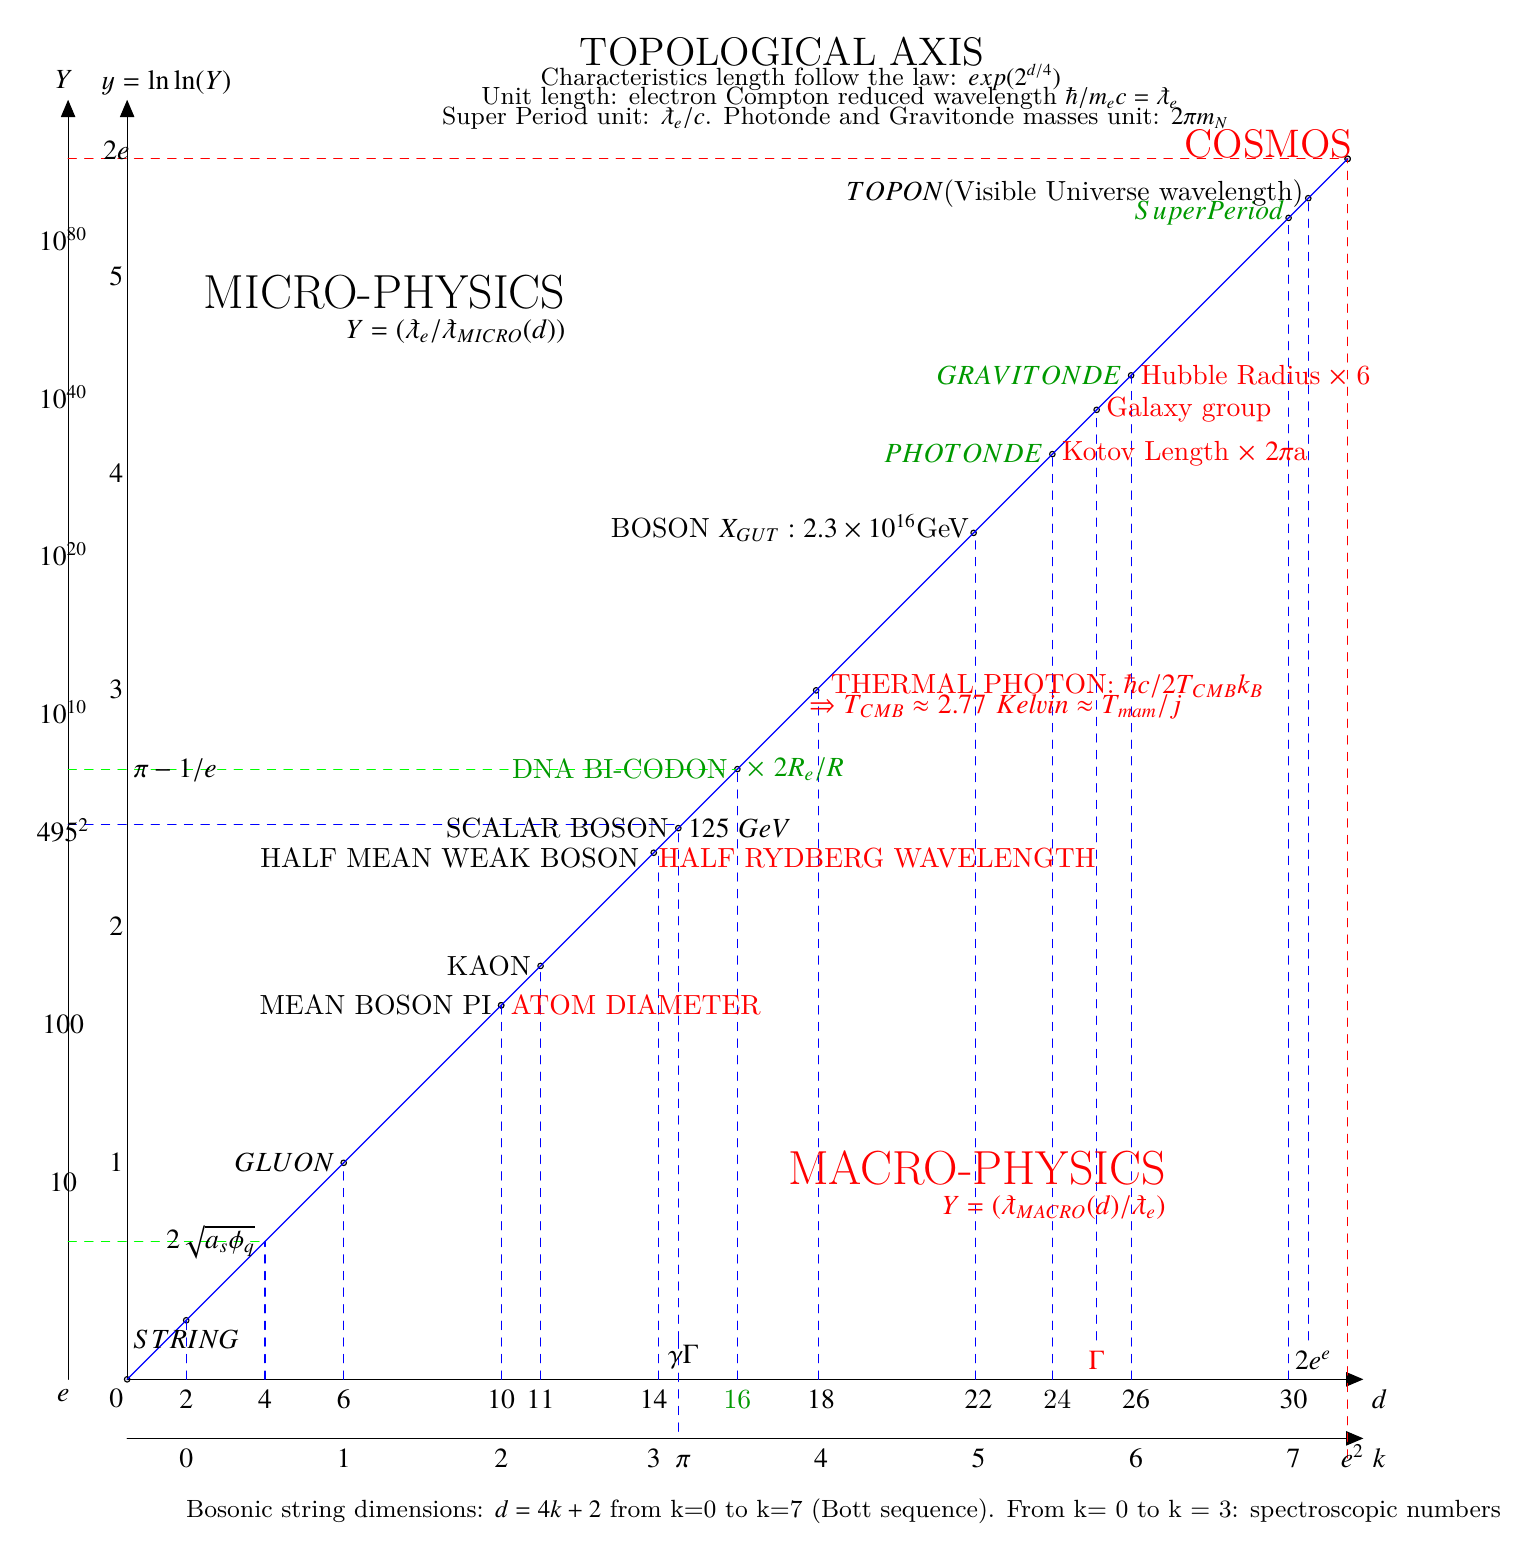
\begin{tikzpicture}[line cap=round,line join=round,>=triangle 
45,x=0.25cm,y=0.25cm]

\tkzDefPoint(-31.0,-31.0){A} %\tkzDefPoint(5.,3.43){B} \tkzDefPoint(5.,0.){C} \tkzDefPoint(31.0,31.0){Y}
\tkzDefPoint(-28.0,-28.0){B}
\tkzDefPoint(-20.0,-20.0){C}
\tkzDefPoint(-12.0,-12.0){D}
\tkzDefPoint(-12.0,-12.0){E}
\tkzDefPoint(28.0,28.0){F}
\tkzDefPoint(-4.25,-4.25){G}
\tkzDefPoint(4.0,4.0){H}
\tkzDefPoint(12.0,12.0){I}
\tkzDefPoint(-3.0,-3.0){J}
\tkzDefPoint(16.0,16.0){K}
\tkzDefPoint(18.25,18.25){L}
\tkzDefPoint(20.0,20.0){M}
\tkzDefPoint(29.0,29.0){N}
\tkzDefPoint(-10.0,-10.0){P}
\tkzDefPoint[color=red](31.0,31.0){Q}
\tkzDefPoint(31.0,31.0){Y}
\tkzDrawPoints(A,B,C,D,F,E,G,H,I,J,K,L,M,N,P,Q,Y)
%\tkzMarkRightAngle(A,D,C)
%\tkzLabelPoints[text=red,right](G,H)
%\tkzMarkAngle[fill=blue!40,size=1.4cm,opacity=.5](C,A,B)
%\tkzLabelAngle[pos=1.6](C,A,B){$\theta$}
\tkzDefMidPoint(A,Y) \tkzGetPoint{BI-CODON}
\coordinate (center) at (BI-CODON);
%\tkzLabelPoints[below,color=green](BICODON)
\tkzDrawPoints(BI-CODON)
\draw [->] (-31.0,-31.0) node[left]{} -- (-31.,34.) node[right]{}; % scale Y
%\draw [->] (31.0,-31.0) node[left]{} -- (31.,31.) node[right]{}; % 
\draw [->] (-31.0,-31.0) node[left]{} -- (31.8,-31.0) node[right]{}; % scale d
\draw [->] (-31.0,-34.) node[left]{} -- (31.8,-34.) node[right]{};   % scale k
\draw [->] (-34.0,-31.) node[left]{} -- (-34.,34.) node[right]{};   % scale Y'
%%% Blue Dashed Horizontal lines
\draw [-,color=green,dashed] (-34.0,-24.) node[left]{} -- (-24.,-24.) node[right]{};   % \sqrt{a_s} horizontal line
\draw [-,color=blue,dashed] (-34.0,-2.8) node[left]{} -- (-2.8,-2.8) node[right]{};   % Scalar Boson horizontal line
\draw [-,color=green,dashed] (-34.0,0.) node[left]{} -- (0.,0.) node[right]{};   % bicodon horizontal line
\draw [-,color=red,dashed] (-34.0,31.) node[left]{} -- (31.,31.) node[right]{};   % Cosmos horizontal line
%%% Blue Dashed Vertical lines
\draw [-,color=blue,dashed] (-28.0,-31.) node[left]{} -- (-28.,-28.) node[right]{};   % String vertical line
\draw [-,color=blue,dashed] (-24.0,-31.) node[left]{} -- (-24.,-24.) node[right]{};   % \sqrt{a_s} vertical line
\draw [-,color=blue,dashed] (-20.0,-31.) node[left]{} -- (-20.,-20.) node[right]{};   % Gluon vertical line
\draw [-,color=blue,dashed] (-12.0,-31.) node[left]{} -- (-12.,-12.) node[right]{};   % ATOM DIAMETER vertical line
\draw [-,color=blue,dashed] (-10.0,-31.) node[left]{} -- (-10.,-10.) node[right]{};   % Kaon vertical line
\draw [-,color=blue,dashed] (-4.0,-31.) node[left]{} -- (-4.,-4.) node[right]{};   % Half Mean Weak Boson vertical line
\draw [-,color=blue,dashed] (-3.0,-29.) node[left]{} -- (-3.,-3.) node[right]{};   % Scalar Boson vertical line
\draw [-,color=blue,dashed] (-3.0,-29.) node[left]{} -- (-3.,-34.) node[right]{};   % \gamma\Gamma->\pi vertical line
\draw [-,color=blue,dashed] (0.,-31.) node[left]{} -- (0.,0.) node[right]{};   % Bicodon vertical line
\draw [-,color=blue,dashed] (4.1,-31.) node[left]{} -- (4.1,4.1) node[right]{};   % Thermal Photon vertical line
\draw [-,color=blue,dashed] (12.1,-31.) node[left]{} -- (12.1,12.1) node[right]{};   % Boson X GUT vertical line
\draw [-,color=blue,dashed] (16.,-31.) node[left]{} -- (16.,16.) node[right]{};   % Photon vertical line
\draw [-,color=blue,dashed] (18.25,-29.) node[left]{} -- (18.25,18.25) node[right]{};   % Galaxy group vertical line
\draw [-,color=blue,dashed] (20.0,-31.) node[left]{} -- (20.0,20.) node[right]{};   % Gravitonde vertical line
\draw [-,color=blue,dashed] (28.0,-31.) node[left]{} -- (28.0,28.0) node[right]{};   % Super Period vertical line
\draw [-,color=blue,dashed] (29.,-29.) node[left]{} -- (29.,29.0) node[right]{};   % Topon vertical line
\draw [-,color=red,dashed] (31.0,-35.) node[left]{} -- (31.,31.) node[right]{};   % Cosmos vertical line

\draw[color=blue] (A) -- (Y);
\node [anchor = text=blue] at (-8.,35.75) {\Large{TOPOLOGICAL AXIS}};
\node [anchor = text=black] at (-10.,34.75) {\small{Characteristics length follow the law: $exp(2^{d/4})$}};
\node [anchor = text=black] at (-13.,33.75) {\small{Unit length: electron Compton reduced wavelength $\hbar /m_e c=\lambdabar_e$}};
\node [anchor = text=black] at (-15.,32.75) {\small{Super Period unit: $\lambdabar_e/c$. Photonde and Gravitonde masses unit: $2\pi m_N$}};
\node [anchor = text=black] at (-28.,-38.0) {\small{Bosonic string dimensions: $d=4k+2$ from k=0 to k=7 (Bott sequence). From k= 0 to k = 3: spectroscopic numbers}};
\node [anchor = east,text=red] at (31.75,31.75) {\Large{COSMOS}};
\node [anchor = south] at (-28.,-33.0) {$2$};
\node [anchor = south] at (-28.,-36.0) {$0$};
\node [anchor = north] at (-28.,-28.0) {$STRING$};

\node [anchor = south] at (-24.,-33.0) {$4$};
\node [anchor = east] at (-24.,-24.0) {$2\sqrt{a_s\phi_q}$};
\node [anchor = south] at (-20.,-33.0) {$6$};
\node [anchor = south] at (-20.,-36.0) {$1$};
\node [anchor = east] at (-20.,-20.0) {$GLUON$};
\node [anchor = south] at (-12.,-33.0) {$10$};
\node [anchor = south] at (-10.,-33.0) {$11$};
\node [anchor = south] at (-12.,-36.0) {$2$};
\node [anchor = east] at (-12.,-12.) {MEAN BOSON PI};
\node [anchor = west,color=red] at (-12.,-12.) {ATOM DIAMETER};
\node [anchor = east] at (-10.,-10.) {KAON};
\node [anchor = south] at (-4.25,-33.0) {$14$};
\node [anchor = south] at (-4.25,-36.0) {$3$};
\node [anchor = east] at (-4.5,-4.5) {HALF MEAN WEAK BOSON};
\node [anchor = west,color=red] at (-4.5,-4.5){HALF RYDBERG WAVELENGTH};
\node [anchor = south] at (-2.75,-31.0) {$\gamma\Gamma$};
\node [anchor = south] at (-2.75,-36.0) {$\pi$};
\node [anchor = east,color=black] at (-3.0,-3.0){SCALAR BOSON};
\node [anchor = west,color=black] at (-3.0,-3.0){$125~GeV$};
\node [anchor = south,color=black!40!green] at (0.,-33.0) {\textbf{16}};
\node [anchor = east,color=black!40!green] at (0.,0.0) {DNA BI-CODON};
\node [anchor = west,color=black!40!green] at (0.,0.0) {$\times~2R_e/R $};
%\node [anchor = west,color=black!40!green] at (0.,0.0) {$\times$ $2R_e/R\approx \mu^3\approx (\tau/\sqrt{e/2})^2$};
\node [anchor = south] at (4.25,-33.0) {$18$};
\node [anchor = south] at (4.25,-36.0) {$4$};
\node [cross,anchor = west,color=red] at (4.25,4.25){THERMAL PHOTON: $\hbar c/2T_{CMB}k_B$};
\node [cross,anchor = west,color=red] at (3.15,3.15){$\Rightarrow T_{CMB} \approx 2.77 ~Kelvin \approx T_{mam}/j$};
\node [anchor = south] at (12.25,-33.0) {$22$};
\node [anchor = south] at (12.25,-36.0) {$5$};
\node [anchor = east,color=black] at (12.25,12.250){BOSON $X_{GUT}:2.3 \times 10^{16}$GeV};
\node [anchor = east,color=black!40!green] at (16.,16.){$PHOTONDE$};
\node [anchor = west,color=red] at (16.,16.){Kotov Length $\times$ $2\pi$a};
\node [anchor = west,color=red] at (18.25,18.250){Galaxy group};
\node [anchor = south,color=red] at (18.25,-31.0) {$\Gamma$};
\node [anchor = east,color=black!40!green] at (20.,20.0){$GRAVITONDE$};
\node [anchor = west,color=red] at (20.,20.0){Hubble Radius $\times$ 6};
\node [anchor = south] at (16.25,-33.0) {\textbf{24}};
\node [anchor = east,color=black!40!green] at (28.25,28.250){$Super Period$};
\node [anchor = east,color=black] at (29.25,29.250){$TOPON$(Visible Universe wavelength)};
\node [anchor = east,color=black] at (-8.25,24.250){\LARGE{MICRO-PHYSICS}};
\node [anchor = east,color=black] at (-8.25,22.250){$Y=(\lambdabar_e/\lambdabar_{MICRO}(d))$};
\node [anchor = east,color=red] at (22.25,-20.250){\LARGE{MACRO-PHYSICS}};
\node [anchor = east,color=red] at (22.25,-22.250){$Y=(\lambdabar_{MACRO}(d)/\lambdabar_{e})$};
\node [anchor = south] at (20.25,-33.0) {$26$};
\node [anchor = south] at (20.25,-36.0) {$6$};
\node [anchor = south] at (28.25,-33.0) {$30$};
\node [anchor = south] at (28.25,-36.0) {$7$};
\node [anchor = south] at (31.25,-36.0) {$e^2$};
\node [anchor = south] at (29.25,-31.0) {$2e^e$};
\node [anchor = south] at (32.6,-33.00) {$d$};
\node [anchor = south] at (32.6,-36.00) {$k$};
%%% Y AXIS
\node [anchor = north] at (-31.55,-31.0) {$0$};
\node [anchor = north] at (-31.55,-19.0) {$1$};
\node [anchor = north] at (-31.55,-7.0) {$2$};
\node [anchor = north] at (-31.55, 5.0) {$3$};
\node [anchor = north] at (-28.55, 1.0) {$\pi-1/e$};
\node [anchor = north] at (-31.55, 16.0) {$4$};
\node [anchor = north] at (-31.55, 26.0) {$5$};
\node [anchor = north] at (-31.55, 32.4) {$2e$};
\node [anchor = north] at (-29.0,36.0) {$y=\ln\ln(Y)$};
%%% Y' AXIS
\node [anchor = north] at (-34.25,-31.0) {$e$};
\node [anchor = north] at (-34.25,-20.0) {$10$};
\node [anchor = north] at (-34.25,-12.0) {$100$};
\node [anchor = north] at (-34.25,-2.0) {$495^2$};
\node [anchor = north] at (-34.25,4.0) {$10^{10}$};
\node [anchor = north] at (-34.25,12.0) {$10^{20}$};
\node [anchor = north] at (-34.25,20.0) {$10^{40}$};
\node [anchor = north] at (-34.25,28.0) {$10^{80}$};
\node [anchor = north] at (-34.25,36.0) {$Y$};
%% SLOPE
%\tkzLabelSegment[sloped,below,text=black](A,D){Slope $\ln(2)/4$}
\end{tikzpicture}
\caption[Graphics \ref{AxeTopologique}: Topological Axis ]{The main physical characteristics lengths $Y$, with unit length the electron reduced Compton wavelength: $\hbar/ m_ec=\lambdabar_e$, follows the law $exp(2^{d/4})$. This is the extrapolation of the Eddington's Large Number correlations, a reunion of height 2D-1D holographic relations, whose micro-macrophysics imbrication explains the double log, hence the name `Topological Axis'\cite{Sanchez2}. The double natural logarithms $y = ln(ln(Y))$ corresponds to the special string dimension series, which identifies with the spectroscopic series with spin 1/2, where $k$ is the orbital quantum number, $d = 4k + 2$, from $k = 0$ to $k = 7$, characteristics of a Bott octonion sequence. The mean value $d=16$ connects with the DNA bi-codon, decisive in the Holic Cosmology, where $R_e$ is the holographic reduced Cosmos radius and $R$ the Hubble radius. The mammal temperature $T_{mam}\approx j T_{CMB} $ connects directely with the Cosmos one $T_{CMB}$ where  $j = 8\pi^2/ln2$ is the scale factor \cite{Sanchez3}. The ratio $R_e/R = pH/a^3$ is connected with the gauge couplings in Eq(9) while $\phi_q \approx 16/\pi_q^2$ is close to the Golden Number. $\Gamma=\gamma a/\pi$ is the Atiyah constant \cite{Atiyah}. The Kotov length is $ct_{nl}$. The Nambu mass, central in Particle Physics, is $m_N = a m_e$. In this rehabilitation of the Bosonic String Theory, the Universe appears as the final gauge boson in the Cosmos:  U (k = 7), GUT (k= 5), Weak (k=3), Gluon (k=1). }

\label{AxeTopologique}

\end{table}




\begin{table}
%\label{tab:6:table6}
\caption[Table \ref{tab:6:table6}: 56 Hubble radius formulas]{56 formula for the Hubble radius $R$}
\label{tab:6:table6}
  \hskip-2.0cm\begin{tabular}{lll}
    \toprule
    %\multicolumn{3}{c}{}     \\
    \cmidrule(r){1-3}
    Formula     & Value (Gly)  & Remarks \\
    \midrule
 
 $ 2\hbar^2/Gm_em_pm_H $ & 13.81197676 & \underline {Gravitational Hydrogen Molecule radius} \cite{Sanchez2}\\ 
 $ (H/p_t)~R_{1H}$ & 13.81197676 & From mono-atomic star limit radius  $R_{1H}$ \cite{Davies} \\
 $ \lambdabar_w ~(t_{nl}/t_e)^2$ & 13.81197676 & Identification predicting $t_{nl}\approx 9600.591457 s$~(Eq.(5)) \\
 $ (\lambdabar_{p} \lambdabar_{H})^{1/2} ~(WZ)^4$  & 13.81197676 & Symetrising the standard relation $a_G \approx W^8$ \cite{Rees}~~~~ $(WZ)^4\approx (2a_w)^3 (a/\pi)^4 (\Phi ln \Phi)^2$ \\
 $\lambdabar_{e} ~2^{128}/d_e^2(m_H/m_p)^6$  & 13.81197676   & From the Combinatorial Hierarchy Lucas Large Number \cite{Bastin}\\
  $(n_tp_W/1836p)^{1/2}\lambdabar_{e} (2^{18}/\pi \sqrt a)^{10}$  & 13.811977   & From $(2g_3)^{21} \approx s_{65}/2\pi$; $p_W = 6\pi^5$ and $s_{65} \approx (2\pi)^2 \sqrt a$\\
  $ (1/g_0) ~\lambdabar_H ~(R_C/2^{128}l_P)^{1/2} $  & 13.811978 & From $1/g_0 = 1+g_1^2+g_2^2\approx2a^3/pp_G$, with $p_G = P/2^{127/2}$\\ 
 $ (\lambdabar_{p} \lambdabar_{H})^{1/2}~ a_w^{7/2}~ a/2\sqrt 5 $  & 13.811978 & From $(WZ)^8 \approx a^2a_w^7/20$\\
 $ \lambdabar_e ~(p_{hol}/p)^2~ e_3 ^{\sqrt a/2}$ & 13.81198 & From a liaison between $e_3 = exp(exp(e))$ and $p_{hol}^2 = 4a^3/3$   \\
 $ \lambdabar_{e} ~(2\pi/3)^{120} (H/p_t^{10}p_t/p_W)^2$ & 13.81199 & \underline {With the unifying geometrical unit $2\pi/3$ (Eq.(64)}   \\
 $ (32 \beta^2 /\pi^3) ~\lambdabar_{CMB}^3/ \lambdabar_Z^2$ & 13.81200 & From the holographic relation $2\pi R/\lambdabar_e \approx (4\pi/3) (\lambdabar_{CMB}/\lambdabar_{H_2})^3$ \cite{Sanchez2}\\  
 $(H/p_W)~(2\pi^2 a^3)^5~ \lambdabar_{e} $ & 13.81196 & with $p_W = 6\pi^5$, 5D holography in the gravitational Hydrogen molecule \cite{Sanchez3}  \\
  $\lambda_{p} ~(pH)^{3a_s/4}  $ & 13.81193 & Confirms the strong coupling $a_s$  \\
  $ 4 ~a^4 ~\lambdabar_{e} ~(m_{bc}^{(0)}/m_H)^9 (p_t/p_W)^2  $ & 13.81196 & DNA bi-codon mass as calculation basis  \\
  $ \lambdabar_{e}~ (WH/Zp)^{1/2}~C_y^{(0)32}/6f(26)   $ & 13.81195 & Cytosine topologic pertinence  $C_y^{(0)} \approx f(10)= f(26)^{1/16} $  \\
  $ \lambdabar_{e}~ (N_{ph}  ~(n_t/p_t)^2/\pi \sqrt{g_0})^{1/7} $ & 13.81197 & With $N_{ph}$ the Cosmos photon number, confirms that the Universe is a cosmic boson \\
 $R_C ~(a_se^{2/a}210^{-210})^{1/8}$  & 13.81198    & With the holic number $210^{210}$, confirming the couple Universe- Cosmos \\
 $ l_{P} ~\sqrt a ~(\mu^{\mu}~Wp/ZH)^{1/8}$  & 13.81198 & Shows the pertinence of the computational term $\mu^{\mu}$   \\
  $(H/p_t)~(ad_e/137)^4 ~R_{R_c,M_N} $ & 13.81203    & From the geo-adimensional Cosmos-Universe (Fig.1)\\
 $(137\beta/a)^2~R_c~R_e~l_P^2/a_w l_{nl}^2\lambdabar_{bc}^{(0)}$ & 13.81194    & From the Holic Principle, with the reduced wavelength of the DNA bi-codon. \\
$(\pi ~a/6\times 137) ~\lambdabar_e ~(1/g_0)^{210} $ & 13.81185 & From $(1/g_0) \approx 2R/R_e \approx (R/\lambdabar_e)^{1/210}$ (Eq. (14)) \\   
 $ (136/137)~2~l_{nl}~a^3~f(16)$  & 13.8120    & With the central value $f(16) = e^{16}$ \\ 
  $ (137^4/ap_t^2)~\lambda_{WCMB}~(e^a/4\pi)^{1/2}$  & 13.8120    & Confirms the Wien CMB wavelength, from $4\pi (R_e/\lambda_{WCMB})^2 \approx e^{a}$ \\  
$ \lambdabar_{e} ~ (1/q)^{3\pi a_s}/496$  & 13.8124    & Confirms the strong coupling $a_s$ and the electric charge $q$ \\ 


%$ l_P e^a \sqrt o ~ \lambdabar_{H})^{1/2} ~a_w^4~ a^{14}/137^{16}$  & 13.8132    &  $o = (o_1+o_2)/2$ mean mass of DNA couples aT and GC \\

$ l_P e^a \sqrt o $  & 13.8132    &  $o = (o_1+o_2)/2$ mean mass of DNA couples aT and GC \\

 $(\lambdabar_{p}~ \lambdabar_{H})^{1/2} ~a_w^4~ a^{14}/137^{16}$  & 13.8119    &  $137,a,a_w$ as computation basis \\
  $(2a/137)~q^2 ~Z^{16} \lambdabar_{p} \lambdabar_{H}/2^{127}\lambdabar_{e} $  & 13.8221    & Cosmic role of electric charge $q = g_1 \cos \theta = g_2 \sin \theta$  \\
 $4~o_2~\sqrt Z~ \lambdabar_{e}\lambda_{CMB}/l_P     $  & 13.8129    &Confirms the cosmic thermal bath and the couple GC with atomic mass $o_2$    \\
 $ (H/p_t)~(Gm_n/c^2) ~(10N_{Ed}/3)$ & 13.8125 &\underline{ From the Eddington Number $136 \times 2^{256}$ and the gravitational parameter 10/3} \cite{Sanchez3}  \\
 $ R_e ~({f(-2)}/exp(exp(-g_1))^{128}/d_e^3$  & 13.8117    & Symmetry $R_e/R$ associated to symmetry f(2)-$g_1$  (string-SU(1) gauge coupling)     \\
 $ 2~\lambdabar_{e} ~((1836+s_{65})/2)^{\sqrt a} $  & 13.8123 & Pertinence of the symmetry 1836-1848 (Eq.(25))\\
  $ (\lambdabar_{p}~ \lambdabar_{H})^{1/2} ~(P/a^{13/2})^5/2\sqrt 5 $  & 13.8124 & From the relation $a_w^7 \approx P^{3+7}/a^{(7 + 127)/2}$ \cite{Sanchez3}\\
  $6~(\lambdabar_{e}^2/\lambdabar_w)~(a/\pi)^{16}$  & 13.8124    & From the Topologial Axis: $f(18)\approx H^3 \approx (a/\pi)^4 (6^{1/2}a_w)^{1/2}$  \\
  $   (1/q)^{3\pi a_s}~\lambdabar_{e}/496$  & 13.8124    & Confirms the strong coupling $a_s$ and the electric charge $q$  \\ 
  $4~\lambdabar_e~a~ W~Z~ F ~ (p_tH)^3$  & 13.817    & Shows a symmetry $a~ W~Z~ F$ \\
  $4~l_{nl}~ (p_t~H/d_e)^2$  & 13.815    & Confirms the non-local Kotov length \\
 $\lambdabar_e ~(2/d_e^8)^{128}/(2g_0-1)$  & 13.815    &  From the Combinatorial Hierarchy Lucas Large Number [12] \\ 
  $ 2~\lambdabar_{H}2^{210} ~(a_w/P)^2  $ & 13.811 & Pertinence of the holic term $2^{210}$ \\
  $ \lambdabar_e ~e^a/p_t^6\Gamma$ & 13.811 & Confirms the pertinence of the Atiyah constant $\Gamma$  \\
  
  $ l_{P} ~ (1/g_1)^a (43H/p_t)^2$  & 13.811    & Base $1/g_1$  \\
  
  
  $ l_{P} ~(\pi 210^{210}/8)^{1/8}$  & 13.81    & Pertinence of the holic term $210^{210}$  \\
 $R_e~ a^a/\Pi_{heur}$  & 13.81    & With the product of the 20 happy sporadic groups $\Pi_{heur}\approx e^{674.5210287}$  \\
$ 2~\hbar^2/Gm_em_pm_n $ & 13.80 & \underline{c-free dimensional analysis} \cite{Sanchez4}  \\
 $(\Pi_+/\Pi_0) \lambdabar_{e}~ e^{1/(g_0-g_2)}$ & 13.82 & Confirms the pertinence of $g_0$ and $g_2$  \\
 $l_{nl}~2~p_t^3~H/d_e $ & 13.82 & $p$ and $H$ as computation basis  \\
 $ (\lambda_{CMB}/(j+1))^2/l_P$ & 13.80 & Central role of mammal temperature: $T_{mam}\approx j T_{CMB}$, with $j = 8\pi^2/ln2$ \\
  %$ 2~ \lambdabar_{e}~ (1/sin\theta)^{10d_e\sqrt {137}} $ & 13.80 & Corresponds to $(1/sin\theta) \approx 3/\sqrt2 \approx p^{1/10}$   \\
  $ \lambdabar_{e} ~\pi^{155/2}$ & 13.80 & $\pi$ calculation basis: $2^{1/155} \approx \pi^{1/16^2}  \approx (2\pi)^{1/3\times 137} $  \\
  $ 2~\lambdabar_{e}~ e_3^{2\sqrt a_s}$ & 13.79 & Basic economic number $e_3 = e^{e^e}$  \\
  $ \lambdabar_{e} ~(6/\pi)^{r_H/\lambdabar_e}$ & 13.78 & $6/\pi$ calculation basis   \\    
 $ g(6) ~\lambdabar_{e} $ & 13.82 & \underline{With the reduced topological function} $g(k) = exp(2^{k+1/2})/k$, for k = 6, d = 26  \\
 %$ 2~l_{nl}~(a\mu)^3 $ & 13.84 & Confirms the non-local Kotov length \\
 $ (2l_{nl}^3/r_e)^{1/2}$  & 13.75    & 2D-3D Holography with the non-local length $l_{nl}$ \\
  $ (r_e^2R_C)^{2/3}/l_{nl}$  & 13.75    & Confirms the Cosmos non-locality \\
 $ (2~\lambdabar_{e}/3) ~(\lambdabar_{CMB}/\lambdabar_{H_2})^2$ & 13.90 &  \underline{2D-3D holography in the hydrogen molecule}\cite{Sanchez5} \\   
   $ (4~\pi ~\lambda_{CMB})^4/r_H^3$ & 13.78 & Confirms the invariant CMB \\ 
    $ (l_P/2)~(\lambdabar_{CMB}^2\lambdabar_p/\lambdabar_{CNB}r_e^2)^6$  & 13.7    & Complementarity of photons and neutrinos backgrounds \\
 
 %\bottomrule
  \end{tabular}
\end{table} 
 

\subsection{The Classical Universe Radius and the Cosmic Gravity-CMB-Micro-physics connection}
The standard theory associates conservation law with symmetry. However, a conservation law can be seen as the result of a computation. Considering that the Universe is a computing black-hole of radius $R$, this introduces the length $(Rl_P^2)^{1/3} \approx 10^{-15} $ m \cite{Sanchez5}. The identification with the \textit{invariant} electron classical radius defines the Classical Universe Radius $R_e$. \textit{It is the radius eliminating $c$ between the classical electron radius and the Planck length formula. This radius presents a very precise dramatic holographic property involving the CMB Wien wavelength}:

\begin{equation}
 \left\{
    \begin{array}{ll}
    R_e = 2r_e^3/l_P^2 = 2 \hbar^2/Gm_N^3 ~~~~~~~~~~~~ M_N = m_P^4/m_N^3 \\
   4\pi(R_e/\lambda_{WCMB})^2 \approx e^a
    \end{array}
\right.
\end{equation}

    
where $M_N = R_ec^2/2G $ is the associated critical mass, implying the Nambu mass $m_N = am_e$, central in particle physics \cite{Nambu}. The OCP introduces the coupling $g_0$, the geometric extension of the Weinberg triangle \cite{Taylor}, $1/g_0 = 1+g_1^2 +g_2^2 = 1 + (Z/H^{(0)})^2$. With the BE-Higgs scalar boson mass ratio, by respect to electron:  $H^{(0)} = 495^2$ (125.208 GeV)\cite{Sanchez2}, $g_0$ identifies with $(p_G/H)R_e/2R$ and $g_1g_3/g_2$, involving $G$ through $p_G = P/2^{127/2}$ (from the Combinatorial Hierarchy \cite{Bastin}). The economic number of order 4, with alternate signs (+,-,+,-) is very close to $g_1$, and its fourth root to $1/2g_0$, while $g_1$ connets twice with the string parameter f(2). The following relations are observed: 
\begin{equation}
 \left\{
    \begin{array}{ll}
    1/g_0 = 1+g_1^2 + g_2^2 = 2a^3/pp_G \approx 2 g_1^{1/4}(pp_W)^{1/2}/H ~~~~~~~~~~~~~\rightarrow~~~    (1/2g_0)^4 \approx g_1 \approx e^{-e^{e^{-e}}} \approx \sqrt2/f(2) \approx f(2)e^{-W_5/2}\\
   tg \theta =  g_1/g_2 = g_0/g_3 \approx 9\mu/\tau \approx (\mu^3/\tau^2)^2 ~~~~~~~~~~~~~~~~~~~~~~~~~~~~~~~\rightarrow~~~   1/lng_3 \approx 5 + 1/137 = 2\times7^3/137\\
   q = g_1 cos \theta = g_2 sin \theta = (4\pi_q/a)^{1/2} \approx y\Pi_+/2d_e\sqrt F  ~~~~~~~~~~~~~~~\rightarrow~~~  3^{11-1}\approx 6(2\pi_q)^5 \approx \pi a^2\\
   f(2) = e^{\sqrt 2} \approx ((\mu +2)/3)^{1/3} \approx (p_W/p_t)^4 4a_s^2~\mu/ \tau \approx (p_t/p_W) (2/g_1e^2)^{1/3}/g_0 g_1\\
   q \approx 3/\pi^2 \approx (3/10)\sqrt(6F)/p_{00} \approx (6^2/\beta d_e)^{-1/3}\approx (6\mu/137g_0\Gamma)^2 \approx 2 a^{1/4} (8/5)^8 \tau/pH \\
   1/g_0 = (H/p_G) 2R/R_e \approx 2(g_1\tau/mu)^{1/2}/\pi \approx (H/2g_1 \sqrt {p_tp_W})^4 \approx 2(H/p_t)(\beta \sqrt {a_s}/W_5)^{1/2}\\
   495 \approx (H/H-p_t)g_1g_2g_3 \approx a_s (\tau/\mu-1)/g_1g_2g_3 \approx a_s^2 \sqrt{n_tH}/\Pi_0 \approx n_t s_{65}/8\pi \Pi_+ \\
   495 \approx (137/a)^4\Delta_{Ed}/g_1g_0g_3 \approx p^2\Pi_0/K_0pa_{Ed} \approx (5/W_5) \tau \Pi_+/2K_+\\
   K_n = (32 \xi(3) /3\pi)^{1/2} R l_P/(\lambdabar_{CMB}^3 \lambdabar_H)^{1/2} \approx K_E (1-1/12^2)^{-1/2} 
    \end{array}
\right.
\end{equation}
Note that the \textit {a-dimensional} electric charge $q$ is tied to the Mirimanoff prime 11 \cite{Mirimanoff}, showing the connection supersymmetry-supergravity: 10 = 11 - 1. The small difference between $g_0$ and $g_2$ induces formula in the Hubble and Cosmos Tables. The dimension 11 in the Topological Axis is tied to the Kaon. Indeed, the "strange" mesons $K_0 \approx 973.784$ and $K_+ \approx 966.119$ appears in liaison with Eddington's parameters and the Wien factor $W_5/5 = 1-e^{-W_5}$. \textit{This means there is a symmetry between radiation and matter, totally unexpected in the present standard theory. The underlined overwhelming correlation in Table 2 has the same form than that of Eddington: $\sqrt{M/m_e} = R/2\lambdabar_H$, equivalent to the definition of $R$ in Eq. (5)}, becoming very precise (0.1 ppm) in the above last relation of Eq.(9).


\subsection{The Tachyonic Holographic Cosmos}
The radius $R_e$, about 30\% larger than $R$, was identifed to the holographic reduced Cosmos radius \cite{Sanchez3}, defined by the Bekenstein-Hawking entropy of the $R_e$-radius sphere \cite{Bekenstein}: $\pi (R_e/l_P)^2 = 2\pi R_C/l_P$, so:   
 \begin{equation}
R_c = R_e^2/2l_P \approx 2^{128} l_P (Rg_0/ \lambdabar_H)^2 \approx 9.075773 \times 10^{86} m 
 \end{equation}
 \textit{The Table \ref{CosmosTable} presents 56 simple formula confirming this Cosmos radius $R_c$.} In particular, there is the dramatic geometrical property, the "Geo-adimensional Cosmos-Universe couple" (Fig.1): 
\begin{equation}
(ln(R_c/\lambdabar_e))^2 \approx (ln(M_N/m_e)^2 + 2(ln(R/\lambdabar_e))^2
\end{equation}

where the 2 factor comes from \textit{the local character of the speed $c$} \cite{Sanchez2}. 



\begin{table}
\caption[Table \ref{CosmosTable}: 56 Cosmos radius formula]{56 formula for the Cosmos radius $R_C$}
\label{CosmosTable}
  \hskip-2.0cm\begin{tabular}{lll}
    \toprule
   % \multicolumn{3}{c}{}                   \\
    \cmidrule(r){1-3}
    Formula     & Value ($10^{86}$m)  & Remarks \\
   \midrule
 
 $ R_e^2/2l_P $ & 9.07577 & \underline {1D-2D Holographic Extension of $R_e$} \cite{Sanchez2}   \\
 $ \lambdabar_e ~ exp(exp(exp(exp(exp(-g'_2)))))  $ & 9.07577 & The final log of $R_c/\lambdabar_e$ is a SU(2) coupling: $g'_2 \approx W/(495^2+(\tau/\mu)^2)$  \\
 $ (\lambdabar_{W}\lambdabar_{Z})^{1/2}e^{1/(a-9)} ~ exp(exp(exp(exp(exp(-g_0)))))  $ & 9.07579 & From the connections $g_0 \approx g_2$ and $a - 9 \approx 2^7$ \\
 
 $ R(1/g_1)^a/3(p_W/a)^2  $ & 9.07582 & Base $1/g_1$. Specifies the celerity ratio $R_C/R = C/c$ \\
 
 $ e^{210}~ R ~(f(16) e^{e^6} 9\mu/n_t)^{-1/6}  $ & 9.07577 & Confirms the role of the central topologic term $f(16) = e^{16}$   \\
 $e^{210}~l_{Wien}\beta (\sin \theta_{1})^4$ & 9.07577 & Confirms the Holic Principle and the CMB invariant temperature   \\
 $ 2^{128}~ l_P (g_0R/\lambdabar_H)^2 $ & 9.07577 & Confirms $1/g_0 = 1+g_1^2 +g_2^2 = 1 + (Z/H^{(0)})^2$  \\
 $ R~p_t (6d_e P^{\sqrt a - 4}/\pi)^{1/3}$ & 9.07574 & From the cosmic atomic mass $M_c/m_H \approx P^{\sqrt a}$  \\
 $ l_P (R_C/\lambdabar_{e})^{g_3}~  (p_G/2a)^{1/2}$ & 9.07574 & Confirms the SU(3) coupling $g_3$ and $p_G$  \\
  $ \lambdabar_{e} ~(a^{3/2}/1837) y^{64a_s}$ & 9.07579 & From $y^{a_s} \approx 3^4 - 1$ \\
 $ \lambdabar_{e} ~14 p_t^2/p_Wn_t (a/4)^{64}$ & 9.07579 & With $p_W = 6\pi^5$ \\
 $ 2\lambdabar_{e}~ (sin_Z \theta_{eff})^{-4} (4a_s)^{64}$ & 9.07777 & Implying a relation between $a$ and $a_s$ \\
 $ l_P ~(\Pi_+/18)3^{256}$ & 9.07586 & Confirms the cosmic base 3 \\
  $ R ~ a^6 ~(12^{32}/P)^{4} 1839/4H$ & 9.07587 & Base 12 \\
  $\lambdabar_{e} ~ (n_t/a^2g_0) ~(3)^{210} $ & 9.07567 & Base 3 \\
 $ g_2\lambdabar_{e}~(60H/61p_t) ~(1/q)^{2^6} $ & 9.07548 & Confirms the electric charge $q$;  $61/60 \approx (n_t/p_t)^{12}$  \\
 $ l_P ~(2/\sqrt5)(80)^{64}$ & 9.07510 & Implying the musical property: $((3/2)^4/5)^{256} \approx 24 (a/137)^{32}(p_t/p_W)^{1/2}$ \\
 $ e^{\mu} ~\lambdabar_{CMB} (R_e/R)^2 (p_t/p_{t0})^4$ & 9.07584 & Confirms the CMB invariant temperature , with $p_{t0}$ = 1836 \\
 $ e^{\mu} ~\lambda_{Wien} e/2\beta^2 \sqrt d_e$ & 9.07575 & Confirms the CMB invariant temperature, through the Wien wavelength\\
 $ e^{\mu} ~l_{phCMB} ~((a-136)p_t/p_{t0})^2$ & 9.07573 & Confirms the CMB invariant temperature, through its photon length $l_{phCMB}$\\
 $ e^{\mu}~ \lambdabar_{e}~ \beta^{1/2} (p_t/n_t)^{1/4} $ & 9.07576 & Confirms the CMB invariant temperature \\
$ 2(a/137\beta)^2 ~l_{nl}^4 ~\lambdabar_{bc}^{(0)}/R_e \lambdabar_el_P^2 $ & 9.07580 & Holic Principle, with the reduced wavelength of the DNA bi-codon \\
 $ l_P ~ (\sqrt{a_w}(a)^2)^{16}  $ & 9.07568 & Bases  $a_w$ and $a_s$, the nuclear couplings  \\
 $ l_P ~ \sqrt{1 + (sin\theta_1)^2}~a^{j/2}  $ & 9.07566 & Base $a$ the electric coupling, with $j$ the scale factor \cite{Sanchez2} \\
 $ l_P ~ (210^{210}(8e)^{-1/2})^{1/4}  $ & 9.07585 & With the Holic central term $210^{210}$  \\
 $ l_P ~ \sqrt2 ~ (p_t/n_t)^6 e^{280}  $ & 9.0767 & Base e  \\
 $ l_P ~ (Zd_e/W) ~7^{12^2}  $ & 9.075 & Base 7  \\
 $ \lambdabar_e ~ 6^{128}/(1+1/\sqrt 2)  $ & 9.075 & Base 6 ; $6/(1+1/\sqrt 2) \approx \mu d_e^2/\sqrt \tau$\\
 $ \lambdabar_e ~ e^{1/2a} 6^{p_G/\sqrt a}  $ & 9.076 & Base 6 \\
 $ 2r_H~ 3^{210}/1830$& 9.076 & Base 3 Holic term, with $ 1830 = u_{30}-1 = (60\times 61)/2 $   \\
 $ l_P ~(g_1g_2g_3)^{-210}~i^{i\pi} $ & 9.062 & Holic Principle with base $(g_1g_2g_3)^{-1}$, confirming the pertinence of $i^{i\pi}= e^{\pi^2/2}$   \\
  $ l_P ~e^{n_t/2\pi}/(g_1g_2g_3\tau/2)^2 $ & 9.062 & Natural base e, with $n_t/2\pi$, the fifth fractionnal of $\pi$ \\
  $ \lambdabar_e ~ (1+1/\sqrt 2)^{6a_s^2+1}  $ & 9.085 & Basee $1+1/\sqrt 2$ \\
  $ \lambdabar_e ~ 5^{2a_s^2+1}/6  $ & 9.082 & Base 5 \\
  $ l_P ~ (7/6)^{(1836p)^{1/2}}/2e^2  $ & 9.085 & Base $7/6 \approx a^{1/32}$ \\
   $ \lambdabar_e ~ ((1/q)^{a}~W/aF)^2  $ & 9.082 & Base $1/q$ \\ 
 $ l_P ~(1/g_1)^{2a}/(g_1g_2g_3)^2p_{hol}^2 $ & 9.081 & Base $1/g_1$,  $p_{hol}^2 = 4a^3/3 $   \\    
 $  l_P~ e^{s_{65}n_tq/2p_W}$& 9.077 & Confirms the terminal Euler number $s_{65} = 1848 $   \\
 $l_P~(p/H) ~(R \Pi_{26}/R_e)^{1/3} $ & 9.076 & With the product of orders of the 26 sporadic groups $e^{674.5210287}$ \cite{Sanchez2}  \\ 
   $  \lambdabar_P ~ (210^{210}/\sqrt(8e))^{1/4}$  & 9.076 & Confirms the Holic Number $210^{210}\approx \tau^{2\mu/3}\approx e^{e2\mu}$  \\
   $ \lambdabar_eg(7)~ (H/p)^2  P/6 $ & 9.076 & With the reduced topologic function for $d = 30: g(7) = f(30)/7$ \cite{Sanchez2}  \\
    $ 24 \lambdabar_e ~ \pi^{210}/a^3 $ & 9.077 & Confirms the base $\pi$ holic term \\
    $ a^2 ~\lambda_{Wien}^4/(p_Kl_P)^3 $ & 9.078 & Confirms $T_{CMB}$ with $p_K = (1+\mu +\tau)/2$ \cite{Koide} \\ 
  $  \lambdabar_e ~  ((3/4\pi)(R_1/\lambdabar_e)^7)^{1/3} $ & 9.078 & From the de photons number, using the mono-electron radius $R_1$ \cite{Sanchez2}  \\
     $  \lambdabar_e ~ 137^{1836/(2\pi)^2}   $ & 9.078 & Base 137\\
  $ \sqrt 3~l_{nl}^3/r_el_P $ & 9.07 & With the non-local length $l_{nl}$  \\
  $ \lambdabar_e~ g(7) ~(a^2p_tp_G)^2 $ & 9.08 &  \cite{Sanchez2}  \\
  $ l_P ~b_3^{210}~a/\pi $ & 9.06 & Holic Principle with base $b_3 = 2 + \sqrt 3$, the Lucas primality test generator \cite{Sanchez5}  \\
   $ l_P ~j^{60}~ e_3^{1/4} $ & 9.06 & Base $j= 8\pi^2/ln2$, the scale factor  \\
 $ (ln(R_c/\lambdabar_e))^2 \approx (ln(M_e/m_e)^2 + 2(ln(R/\lambdabar_e)^2) $ & 9.12 & \underline{c-observable Universe  Cosmos couple} $(R/\lambdabar_e = t/t_e)$ , fig 1   \\
  $  l_P ~ (6/\pi)^{\pi a}  $ & 9.14 & Base $6/\pi$  \\ 
 $ \lambdabar_e~ g(7) ~(\lambdabar_{CMB}/r_H)^3 $ & 9.1 & Confirms the invariance of the thermal background \cite{Sanchez2}  \\
 $ \lambdabar_e ~e^{(u_{30}-1/2)/8} $ & 9.1 & Natural base $e$, with $u_{30} = (60 \times 61)/2 + 1$ \\
 $  (Rl_{nl})^{3/2}/r_e^2 $ & 9.2 & From non-local holography \cite{Sanchez2}  \\
  $  l_P ~ \mu^{\mu R_e/3R}  $ & 9.0 & $\mu$ calculation basis, close to holic base $210$   \\
 
 %\bottomrule
  \end{tabular}
\end{table} 
        
     
\subsection{The Non-Local Period: the Photon and Graviton masses}
The Topological Axis rehabilitates the bosonic part of the string theory which has the apparent imperfection it includes tachyons. In fact, it is rather an advantage in order to explain the quasar non-Doppler oscillation, introducing a non-local period $t_{nl} \approx 9600,06 (2) $ s \cite{Kotov}. Indeed, the ratio of this period and the electron period $t_e = h/m_ec^2$ is precisely given by the elimination of $c$ between the electro-weak constant $a_w$ and the inverse gravitational coupling $a_G = R/\lambdabar_e $: $t_{nl} /t_e   \approx  (a_G a_w)^{1/2}$. This gives a $G$ value precise to $10^{-6}$, compatible with the BIPM $10^{-5}$ precise measurement \cite {Quinn}. This implies that the official value of $G$, \textit{the incongruous mean between incompatible measurements}, is dramatically too small by 8 $\sigma$. By analogy with the practical holography, which is a two-step process, it was introduced a two-step interaction procedure, with \textit{a precursor speed} $C = cR_C/R$ much greater than $c$, leading to the following masses for the photon and graviton \cite{Sanchez2}:

\begin{equation}
 \left\{
    \begin{array}{ll}
        m_{ph} = \hbar/c^2t_{nl}\\
        m_{gr} =m_{ph}/a_w
    \end{array}
\right.
\end{equation}

In the Topological axis, these masses correspond to the special string dimensions 24 (transverse dimensions) and 26 (main dimension), and will be determinant in the following section. Note the relation, precise to 1 ppm, between the Bohr's radius $r_H$ and the relativistic factor $1/\beta = H-p$: $f(24)^{1/26} \approx d_e (r_H/\beta\lambdabar_e)^{1/2}$, showing that the electric parameter $a = (p/H)r_H/\lambdabar_e$ is central in the Topological Axis.


 
\section{The Holic Principle}
The string theory considers space-time as a secondary property \cite{Seiberg}, so the concepts of mass, length and time are, in final, related to pure numbers. Indeed an arithmetic-physical synthesis has been anticipated by the Holic Principle  \cite{Sanchez1}, a simplified form of the Holographic Principle. 

Recall that holistic equations are preferred to differential ones, in order to eliminate free parameters. 
The systematic use of differential equations in the standard physics is the origin of the proliferation of free parameters. 

In any Diophantine equation, this Holic Principle allows to discriminate a temporal ratio $T$, acting by its square, from a spatial ratios $L$, acting by its cube (due to the 3D space). Indeed, \textit {the simplest Diophantine Equation, which implies a 2-dimensional Time}, $T^2 = L^3 = n^6$, with $n$ a natural integer, is the Diophantine form of the third law of Kepler, and implies: $L_n = r_n /r_1 = n^2$ (the Bohr's orbit law) and $T_n = t_n/t_1 = n^3$. Hence, with $v_n = r_n/t_ n$:


\begin{figure}
\centering
\includegraphics[width=5cm,height=6cm]{./figure/triaxis.png}
\caption[Figure \ref{cuboid} MLT A-dimensional cuboid]{\textit{Geo-adimensional Cosmos-Universe couple}, with unit length the Electron Compton reduced wavelength. In a 3D Super-space, logarithms of physical ratios are considered vectors. The Cosmos radius $ R_C$ appears as the norm of the vector using for length and time projections the same value $R/\lambdabar_e = t/t_e$. For the mass projection it is $M_N/m_e$ where $M_N$ is the critical mass in the Cosmos \textit{reduced spherical hologram} of radius $R_e$. This is a dramatic geometrical confirmation (independent of the base for logarithms) of the Extended (2D-1D) Holographic Principle applied to the Bekenstein-Hawking Universe entropy. So the Universe is characterised by the c-equivalence $R/\lambdabar_e = t/t_e$, where $t$ is the Hubble time (no relation with any "Universe age").} 
\label{cuboid}
\end{figure} 

 \begin{equation}
 \left\{
    \begin{array}{ll}
        r_nv_n^2 = r_1v_1^2 = Gm_G \\
        r_nv_n = nr_1v_1 = n \hbar/m_{\hbar}
    \end{array}
\right.
\end{equation}

\textit{These gravito-quantum equations introduce an "hyper-symmetry" between the universal constants $G$ and $\hbar$, by respect to the mass concept: the undefined masses $m_G$ and $m_{\hbar}$}. So, this defines the conceptual trajectories:

\begin{equation}
 \left\{
    \begin{array}{ll}
        r_n = n^2 r_1 \\
        
        r_1 = \hbar^2/Gm_Gm_{\hbar}^2   
    \end{array}
\right.
\end{equation}

With $m_G = m_e^{(red)} = m_em_p/(m_e+m_p)$, the classical electron reduced mass and $m_{\hbar} = m_P/\sqrt a$, this is the Bohr's orbits distribution. The above PSHOB Cosmology includes the following 6 more special cases (Table 6), using the main masses, plus a new one: $m_{bc}$, close to $m_H^2/m_e$, \textit{which identifies with the DNA bi-codon mass}, studied in the next section.

%\begin{equation}
% \left\{
   % \begin{array}{ll}
    
   % m_G = m_e^{(red)};~~  m_{\hbar} = m_P/\sqrt a  ~~~~~~~~~~~~~ \rightarrow r_1 = r_H \\
   % m_G = m_e~~;  m_{\hbar} = m_P  ~~~~~~~~~~~~~~~~~~~~~~~~~ \rightarrow r_1 = \lambdabar_e \\
    
       % m_G = m_{\hbar} = m_N  ~~~~~~~~~~~~~~~~~~~~~~~~~~~~~~~~~ \rightarrow r_1 = R_N/2 \\
        
        
       % m_G = m_{bc} = m_{\hbar}   ~~~~~~~~~~~~~~~~~~~~~~~~~~~~~~~~ \rightarrow r_1 = 2l_{nc} \\
        
       % m_G = a^3 m_P;~~ m_{\hbar}^2 = m_pm_H ~~~~~~~~~~~~~~~~ \rightarrow r_1 = \lambda_{Wn} \\
       % m_G = m_e;~~ m_{\hbar}^2 = m_pm_H ~~~~~~~~~~~~~~~~~~~~ \rightarrow r_1 = R/2 \\
         
        % m_G = m_{bc}R_N/R;~~  m_{\hbar}^2 = m_{ph}m_{gr}    ~~~~~~~~ \rightarrow r_1 = R_C 
    %\end{array}
%\right.
%\end{equation}

%$où $R$ est le rayon de Hubble et $ R_N$ est le rayon \textit{holographique réduit} du Cosmos.

So, the PSHOB Cosmology is tied to the couple $G,\hbar$, while the classical quantum theory uses in fact the "photonde" couple $\hbar,c$, and the gravitation theory the "gravitonde" couple $G,c$. These three couples define the "Trihedra of Constants"(Fig. 2).

\textit{These neologisms 'photonde" and "gravitonde" are introduced to recall that only waves propagate, not the particles: this is a main cause of misinterpretations in quantum physics.}
 
Extrapolating the above simplest Diophantine equation with the prime numbers 5 and 7 which follow the basic prime couple 2;3, the Holic Principle proposes the exponent 5 for a mass ratio, and 7 for a field ratio (note that the lifetime of a particle depends effectively to the power 5 of its mass). So, the general resolution is:

\begin{equation}
T^2 = L^3 = M^5 = F^7 = n^{210}
 \end{equation}
 
 Note that the primes 2;3;5;7 are the terms of the two simplest solutions of the Pell-Fermat equation, which has been connected with the metric equation \cite{Sanchez1}. 
 
 Indeed, the Hubble radius "holic key" is singular, to 15 ppm, while the base 2 is confirmed to 0.3 ppm, and the base 3, to 60 ppb, in the following relations:
  
 \begin{equation}
 \left\{
    \begin{array}{ll}
        (R/\lambdabar_e)^{1/210} \approx 2R/R_e = p_G/Hg_0 \\
    \\
        ((P/F)^4/p_t)^{1/210}\approx 2\\
      \\  
        ((a^2g_0/an_t) R_C/\lambdabar_e)^{1/210} \approx 3
    \end{array}
\right.
\end{equation}

with $p_t$ the proton-electron mass ratio and $n_t$ the neutron-electron mass ratio. Note that 3 is the optimal integer base, the closest integer to $e$ \cite{Hayes}. This is tied to the economic functional definition of $e$, whose square interconnects the main musical ratios, using the primes 2;3;5, while \textit{the ratio 7/6, unknown in classical music, connects with $a$}. Recall that, according to Euler "music is an inconscious calculation":

\begin{equation}
 \left\{  
    \begin{array}{ll}
       x^{1/x} ~~maximal~~ for~~ x = e\\
       \\
        e^2\approx (3/2)^5 \approx (4/3)^7\approx (5/4)^9\approx (6/5)^{11}\approx (7/6)^{13} \approx a^{13/32} \approx \mu^{3/16}\\

    \end{array}
\right.
\end{equation}

\textit{So the base 7 is also pertinent. It is foreseen that special music could use also the base 7. A symmetric use of these four bases 2;3;5;7 explains the above role of the global base 210, so justifies the brute muon mass. }

 

 
\begin{table}
\caption[Table \ref{tab:5:table5}: PSHOB Cosmology.]{PSHOB cosmology (Eq.(12))}
\label{tab:5:table5}
  \hskip-2.0cm\begin{tabular}{lllll}
    \toprule
    %\multicolumn{4}{c}{}                   \\
    \cmidrule(r){1-4}
    $m_G$ & $m_{\hbar}$    & $r_1 = \hbar^2/Gm_G m_{\hbar}^2$  & Precision &Arithmetic Property \\
    \midrule
    
    $m_e$ & $m_P $ & $\lambdabar_e$: Electron reduced wavelength   & exact & \\
    $m_e^{(red)}$ & $m_P/\sqrt a $ & $r_H$: Bohr's radius   & exact & $ r_H/\lambdabar_e \approx 137 = 2^7+2^3+2^0 $\\
    $m_N $ & $m_N$   & $R_e/2$: half cosmos reduced holographic radius  &  exact & $R_e/\lambdabar_e \approx (3^3)^{3^3}$ \\
    $m_{bc}^{(0)} $ & $m_{bc}^{(0)}$   & $2l_{cc}$: double non-local length & $-6.3 \times 10^{-3}$ & $ l_{cc}/\lambdabar_e \approx \pi^{50}$  \\
    $m_Pa^3 $ & $\sqrt {m_pm_H}$  &$\lambda_{Wn}$: Wien CMB wavelength (thermal background) & $-3.2 \times 10^{-4}$ &$\lambda_{Wn}/l_P \approx \pi^{64}$\\
    $m_e $ & $\sqrt {m_pm_H}$   & $R/2$: half Universe radius &exact& $R/\lambdabar_e \approx g(6) \approx 2^{2^7}\approx (2R/R_e)^{210}$   \\
    $m_{bc}^{(0)}R_e/R $ & $\sqrt{ m_{ph}m_{gr}}$   & $R_C$: Cosmos radius = $RC/c = (R/2)m_N^3/m_{bc}m_{ph}m_{gr}$ & $4.7 \times 10^{-4} $& $ R_C/\lambdabar_e \approx e^{e^{2e}} \approx 6^{2^7}\approx (2R/R_e)^{64a_s}  $\\
    
  
         
   \bottomrule
  \end{tabular}
\end{table}







\begin{figure}
\label{figure2}
\centering
\begin{tikzpicture}[scale=2, tdplot_main_coords,axis/.style={->,dashed},thick]
%\tkzDefPoint(1.,-1.,0.75){A} \tkzDefPoint(4.9,0.,-0.75){B} \tkzDefPoint(3.12,0.,-1.74){C}
%\draw[step=1cm,gray,very thin] (-4,-4) grid (4,4);
\node[shape=circle,draw,fill=black,inner sep=1pt] (O) at (0,0,0){};
%\node[shape=circle,draw,fill=black,inner sep=1pt] (M) at (1,-1,0){};
\draw[axis] (0, 0, 0) -- (3, 0, 0) node [right] {$G$};
\draw[axis] (0, 0, 0) -- (0, 2, 0.25) node [above] {$\hbar$};
\draw[axis] (0, 0, 0) -- (0, 0, 1) node [above] {$c$};
\coordinate  (d1) at (1,0,1){};
%\coordinate  (d2) at (3,-2,-1){};
\coordinate  (M) at (1,-1,0){};
%\coordinate  (d3) at (0,0,1){};
%\coordinate  (d4) at (0,0,4){};
%\draw [] (d1) -- (d4)--(d2)--(d3)--cycle;

%\coordinate  (t1) at (1,2.,4){};
%\coordinate  (t2) at (-1,2,4){};
%\coordinate  (t3) at (0,2,2){};
%\draw (t1)--(t2)--(t3)--cycle;
%\foreach \d in {1,2,3,4}{
%\draw[color=red] (O)--(d\d);
%}
%\foreach \i in {1,2,3,4}{
%\foreach \j in {1,2,3}{
%\draw[color=red] (d\i)--(t\j);
%}}
\node[color=black!40!green] at (0.,0.5,-0.5) (l){$\mathbf COSMOS, base ~~3$};
%\node at (2.,0.0,1.5) (l){$\mathbf Gravitation$};
\node[color=black!40!green] at (1.,0.25,1.75) (l){$\mathbf UNIVERS, base~~ 2$};
\node[color=red] at (1.,1.5,1.05) (l){$\mathbf PHOTONDE$};
\tkzLabelSegment[sloped,below,text=blue](d1,M){$GRAVITONDE$}
\end{tikzpicture}
\caption[Figure \ref{figure2}: The $\hbar-G-c$ Trihedra]{The Trihedra of Constants $\hbar- G-c$.  The $c$-local visible Universe is a Cosmos bosonic "immergence"}
\end{figure}



\section{The DNA bi-codon}
Using the main isotopes: $~^{1}_{1}H^{(0)} = H,~ ^{6}_{12}C = C^{(0)},~ ^{7}_{14}N = N^{(0)}, ~^{8}_{16}O = O^{(0)},~^{15}_{31}P= P^{(0)}$  \cite{Huang}, the masses of the 4 DNA nucleotides, by respect to the hydrogen mass $H$ are close to the Fermi mass ratio: $\sqrt {a_w/pH} \approx 311.9846$, very close to 312, the $53^{th}$ idoneal Euler number, while the Guanine nucleon number is 329 = 312 + (2+3+5+7), whose importance will appear in the next Section, in relation with the sum of primes $\sigma_n$: 

\begin{equation}
 \left\{
    \begin{array}{ll}
         Cytosine : ~ ~~C_{9}^{(0)}~H_{12}^{(0)}~N_3^{(0)}~O_6^{(0)}~P^{(0)}: ~(289~ nucleons) : ~ C_y^{(0)} \approx 286.8021362 \approx 495 (a^3/n_t^2)^2 \approx WH/4an_t\\
         
     \\    
        
         Thymine : ~~~ C_{10}^{(0)}~H_{13}^{(0)}~N_2^{(0)}~O_7^{(0)}~P^{(0)}: ~(304~ nucleons) :  T_h^{(0)} \approx301.68553403 \approx  \sqrt {a_w}~\Pi_0/H\Pi_+ \\ 
         
         \\
             
         Adenine : ~~~ C_{10}^{(0)}~H_{12}^{(0)}~N_5^{(0)}~O_5^{(0)}~P^{(0)}:~(\underline{313}~ nucleons):  A_d^{(0)} \approx310.6269397 \approx \sqrt {a_w} /p_td_e^{4}\\
         
         \\
        
         Guanine : ~~~~ C_{10}^{(0)}~H_{12}^{(0)}~N_5^{(0)}~O_6^{(0)}~P^{(0}:~(\underline {329} ~nucleons) :   G_u^{(0)} \approx326.4976654 \approx 495~a/(\mu + 1)\approx Zp_t/2H\Pi_+\\
       
    \end{array}
\right.
\end{equation}

The mean masses of the effective couples are close to $H/3 \approx 612.3842155 \approx \Gamma^2/(a-136)$: 

\begin{equation}
 \left\{
    \begin{array}{ll}
        Couple~AT:~~~ A_d^{(0)} + T_h^{(0)} = o_1 \approx  612.312280 \approx (Z/sin\theta)^{1/2} (p_t/H)^{8} \\
       \\
        Couple~ GC:~~~ G_u^{(0)} + C_y^{(0)} = o_2 \approx  613.299802 \approx (Z/sin\theta)^{1/2} (p_t/H)^{5} 
    \end{array}
\right.
\end{equation}

The bi-codon minimal mass uses the three couples AT, so is very close to $Hm_H$. Since $o_2 \approx o_1 + 1$, the other masses are of type $(H+n)m_H$,  with n = 1, 2 or 3: \textit {the DNA seems a base 3 computer, like the Cosmos}.

Note that the number of protons is the same in the couples AT and CG: 320 = 162 + 158 = 150 + 170.

The mean nucleotide mass is $ (o_1 + o_2)/6 \approx 306.4032199$, close to $\pi^5 \approx 306.02$, the sixth part of the Lenz-Wyler proton-electron mass ratio \cite{Wyler} $6\pi^5$, which shows a geometric property: it is the product of the area by the volume of a cube of side $\pi$. The mean DNA bi-codon mass  $m_{bc}^{(0)}/m_H = (6/4)(o_1 + o_2) \approx 1838.418122$ connects very precisely ( 150 ppb, 100 ppb, and 50 ppb) with the following main parameters   329 being the above Guanine nucleon number) and the central term $f(16)= e^{16}$ of the Topological Axis. This connects also with the Relative Radiation Ratio $y$ (5 ppm) and the second Wieferich prime $p_{W2} = 3511$, while $e^{8}$ connects directly with canonical numbers (0.6 ppm):

\begin{equation}
 \left\{
    \begin{array}{ll}
    329 \approx \sqrt Z / 2g_2 \\
        m_{bc}^{(0)} \approx (m_H^2/m_e)(n_t/p_t)^{1/2} \approx (\tau / 3\mu)(329~G_u^{(0)}d_e)^{1/2} \approx m_ee^8 a^{3/2}/d_e \sqrt 2 \approx m_H p_{W2}Z/yF\\
        e^8/8e \approx (a\beta)^2/137
    \end{array}
\right.
\end{equation}
 
\textit{So, the DNA mass establishes the lacking connection (0.1 ppm) between the main masses, the Guanine nucleon number 329, and $f(12)$, the square root of the central value of the Topological Axis $e^{16} = f(16)$}, which shows also the following Keplerian holic relation, implying the leptons ratios: 

\begin{equation}
e^{16} = f(12)^2 \approx (f(4(1+\sqrt 2))^3 ~~~~ \rightarrow  f(4(1+\sqrt 2) = exp(2^{1+\sqrt 2}) \approx \mu ~~~;~~~ f(12) = e^8 \approx 6\tau/7
 \end{equation} 

where $(1+\sqrt 2)$ is the Pell-Fermat generator. From Eq.(18), $a^{1/32}\approx 7/6$, this implies the terminal term $f(32)$ of the Topological Axis. The analysis shows, to 4 ppm:
\begin{equation}
(\tau -1)^{32}/f(32) \approx a^2/137
 \end{equation}
 
 \textit{So, the terminal dimension 32 of the Topological Axis is associated to $\tau$, the terminal lepton. The number three of particle families is therefore confirmed}. The associated nucleotide to the Guanine is the Cytosine, which is clearly tied with the topological function f(10), giving rise to a formula in the Hubble Table. The other couple (AT), is associated with the Fermi constant. 
 
 One observes the direct correlation implying \textit{the product} of the nucleotide mass ratios: 
 
 \begin{equation}
4d_e G_u^{(0)} C_y^{(0)} \approx 4d_e A_d^{(0)} T_h^{(0)} \approx (H/3)^2 \approx H^{(0)}/g_0 = H^{(0)} + Z^2/H^{(0)}
 \end{equation}
 
 confirming the pertinence of the hypothesis Eq.(9.1) defining  $g_0$. This induces the symmetrical relation implying $s_{65} = 1848$, the last known Euler idoneal number. Note that these numbers 1836 and 1848 are the $34^{th}$ and $35^{th}$ areas of integer-sided triangles whose area equals 6 times their perimeter (A332879 in OEIS):
 
\begin{equation}
 \left\{
    \begin{array}{ll}
        H^{(0)} + Z^2/H^{(0)} \approx (H/3)^2\\
        H^{(0)} + W^2/H^{(0)} \approx (s_{65}/\pi)^2
    \end{array}
\right.
\end{equation}

\textit {The standard central importance of the scalar BEH boson is thus confirmed}. However, its standard interpretation of bringing mass to Zero-mass particle must be reconsidered. Indeed, firstly, the mass concept is necessary in the above $\hbar-G$ symmetry, and secondly, the photon and graviton masses proved to be central in the above Holic Cosmology. 

According to Eddington \cite{Eddington}, the main relation between $a$ and $p_t$ is $a^2 \approx 10 p_t$. With $p_t \approx 6 x$, where $x$ is a nucleotide mass, this corresponds precisely to $a^2/60 \approx 313 = (5^4 +1) /2$, the Adenine nucleus number, which is a prime number. The deviation is pertinent: 

\begin{equation}
 \left\{
    \begin{array}{ll}
        60\times 313 = 137^2 + 11 \approx a^2 + Z/W\\
        a^2 - 137^2 \approx 11 - Z/W \approx \pi^2
    \end{array}
\right.
\end{equation}

\textit{This means that the Cosmos computes the $\pi$ value}, as confirmed in the section 5.5. 


\section{The Multi-Dimensional Crystallography}
The main problem of string theory is the connection between the usual 4D time-space with the favored theoretical dimensions: 26 for the bosonic theory, 24 for the transverse dimensions, 10 for the superstring theory, 11 for the supergravity. 

As recalled above, \textit{conservation is tied to both symmetry and computation}. So, this section is devoted to connections between the Multi-Dimensional Crystallography, the Number Theory and the main particle mass ratios. Carl Hermann \cite {Hermann} calculated the number of crystallographic point symmetries $N_d$ for dimensions from 1 to 8. \textit{This number $N_d$ is the number of monic polynomials (i.e. with first term $1x^d$) with roots on the unit cercle: there must be a connection with the electromagnetic group U(1) of complex numbers with modulus 1.} The Weigel team\cite{Weigel} (Table 7) extended this calculation for higher dimensions, up to $d=70$, focusing on \textit{the positive symmetry number}, noted $K_{d}$, which defines $N_d$ via: 
\begin{equation}
 \left\{
    \begin{array}{ll}
            N_{2n+1}/2 =  K_{2n+1} =  K_{2n} \\
          N_{2n} = K_{2n} + K_{2n-2}
    \end{array}
\right.
\end{equation}
These recurrence rules are non sufficient to defines the series. This implies to look for specific recurrences, characteristic of the Number Theory and the standard "free parameters", in particular ($a;p_t; n_t$) with closest whole values (137;1836;1839).



\begin{table}
%\label{tab:4:table4}
  \hskip-0.0cm\begin{tabular}{llllllllllllll}
    \toprule
    \multicolumn{14}{c}{Table 7 : Multi-dimensional Crystallography and Number Theory}                  \\
    \cmidrule(r){1-14}
      
      \ $E_d$  & $E_1 $ & $E_2$ & $E_3 $& $E_4$ &$ E_5$ &$ E_6 $&$ E_7$ &$ E_8$ & $E_9$ &$ E_{10} $&$ E_{11} $&$ E_{12}$&$ E_{13}$ \\
    \midrule
    $N_d$ & 2 & 6 & 10 & 24 & 38 & \underline{78} & 118 & 224 & \underline{330} & 584 & 838 & 1420 & 2002  \\  
    $K_d$ (positive)  & 1 & 5 & 5 & 19 & 19 & \underline{59} & 59 & 165 & 165& \underline{419} & 419 & 1001 & 1001 \\
     $N_d + K_d$  & 3 & 11 & 15 & \underline{43} & 57 & \underline{137} & 177 & 389 & \underline{495} &  1003 & 1257 & 2421 & 3003 \\
    $\sigma_{(d/2)^2} + \sigma_{(d/2)^2-1}$  & - & 1 & -& 17 & - & \underline{137} & - & \underline{611} & - &  \underline{1839} &   - & 4405 & -\\
    $T_d =\sum_{d-1}^{d+1}K_d$   & 7 & 11 & 29 & \underline{43} & 97 & \underline{137} & 283 & 389 & 749 & 1003 & \underline{1839} & 2421 & 4259 \\
    $S_d=\Sigma_1^d (N_d/2)$   & 1 & 4 & 9 & 21 & 40 & 79 & \underline{138} & 250 & \underline{415} & 707 & 1126 & \underline{1836} & 2837 \\
     $q_d=\binom{3+d}{4}$   & 1 & 5 & 15 & 35 & 70 & 126 & 210 & \underline{330} & \underline {495} & 715 & 1001 &\underline{1365}& \underline{1820}\\
     $Q_d=q_d + d + 3$    & 5 & 10 & 21 & 42 & 78 & \underline{135} & 220 & 341 & 507 & 728 & 1015 & 1380 & \underline{1836}\\
      $u_d = 1 + d(2d+1)$ & \underline {4} & \underline {11} & 22 & 37 & 56 & 79 & 106 & \underline{137}  & 172 & 211 & 254 & 301 & 352 \\
      $u_{2d} $ & \underline{11}  & 37 & 79 & \underline{137}  & 211 & 301 & 407 & 529  & 667 & 821 & \underline{991} & 1177 & 1379 \\
      $u'_d = u_{2 D = 2(d+3)}$ & \underline{137}  & 211 & 301 & 407 & 529 & 667 & 821 & \underline{991} & 1177 & 1379 & 1597 & \underline{1831} & 2081 \\
      13 final idoneals  & \underline {312} & 330 & 345 & 357 & 385 & 408 & 462 & 520 & 760 & 840 & \underline{1320}  & \underline{1365} &\underline{1848}\\
       $ph_{d}$ (A308970)  & 1 & 3 & 11 & 5 & \underline{137} & 7 & 3 & \underline{761}  & 7129 & 11 & 97  & 13 & 29\\
       
       $ph_{d+13}$ (A308970)  & 1049 & 29 & 17 & 37 & 19 & 37 & 7 & $ph_{21}$ & 3 & \underline{761} & 5  & 109 & $ph_{26}$\\
       
      $p_{2^d + 1}$ (A05149)  & 5 & 11 & 23 & 59 & \underline{137} & \underline{313} & 727 & 1621 & \underline{$3673$} & 8167 &17881  & 38891 &84047\\ 
    
     
$p_{d^3}$ (A055875)  & 2 & 19 & 103 & \underline{311}  & 691 & 1321 & 2309 & \underline{$3671$} & \underline{$5519$} & \underline{$7919$}&10957  & 14753 &19403\\ 

$p_{d^2}~~$ (A011757)  & 2 & 7 & 23 & \underline{53}  & 97 & 151 & 227 & \underline{$311$} & \underline{$419$} & 541 & 661  & 827   & 1009 \\
    
 $p_{(d)}^{(16k +5)}$  & 5 & 37 & 53 & 101  & 149 & 181 & 197 & \underline{$229$} & 277 & \underline{$293$} & 373  & 389   & 421 \\
       
 $p_{(d+13)}^{(16k +5)} $  & \underline{$613$} & 661 & 677 & 709  & \underline{$757$}  & \underline{$773$} &821 & 853 & 997  & 1013 &1061   & \underline{$1093$}   & 1109  \\ 
 
  $A298684/5~(d+1)$  & 108 & 132 & 240 & \underline{$264$}  & 324 & 432 &\underline{$612$} & 1116 & \underline{$1224$} & 1344 & 1620  & \underline{$1836$}   & \underline{$1848$} \\
  
A076551-A291138  & 3 & - & - & \underline{$210$} & \underline{$3570$} & - &- & - & - & - & -  & -   & - \\
      
    \bottomrule
  \end{tabular}
\label{tab:7:table7}
\caption{
Crystallographic Ponctual Symmetry Operation numbers $N_d$ and the positive ones $K_d$. With the sum of primes including unity $\sigma_n$ (EOIS A014284): $N_6 = \sigma_{9}$, $K_6 = \sigma_{8}$ and $N_9 = \sigma_{16} + 1$ where $\sigma_{16}$= 329 is the Guanine nucleon number (Eq.(18)). While $N_9+K_9 $ = 495, the square root of the Higgs boson-electron mass ratio, while the sum $N_6+K_6 $ is the Eddington-Atiyah constant 137. Characterizing $9 = (6/2)^2$, the corresponding sum for the supersymmetric dimension $d =10$, is 1839, both the neutron-electron brute mass ratio and the mean bi-codon atomic mass. For $k = 8$, this sum is 611, close to the atomic mass of the couple AT, Eq. (19). The same numbers 137 and 1839 are again given for a triplet combination of nearby $K$, for $d= 6$, and $d = 11$, the supergravity dimension. The sum of $N_d$ for $d = 12$ (half the 24 transverse dimensions) is the double of 1836, the proton-electron brute mass ratio. For the number of compactified dimensions in string theory $d=9$, one observes, moreover, that $N_9 + K_9 = 495$ identifies with the $9^{th}$ pentapope number $q_9$ (EOIS A000332). The relation $S_9 + 4 = K_{10} = p_{9^2} = 419$ seems fundamental, since $419/417\approx F^5/Pa^3$ to ppb precision. The extension of the $13^{th}$ pentapope number, where 13 is half the 26 main bosonic dimensions, is again 1836. The bisection of the Rule 23 Wolfram series shows the dimensions $u_1 = 4$ and $u_2 = 11$, which are those of the usual Space-Time and the Supergravity, with $u_1^2 + u_2^2 = u_8 =137$. Reducing the dimensions by a 2 factor shows that $u_{22}= 991 = 495 + 496$, the third "perfect couple", where 496 is the dimension of the string SO(32) group, while $11 = 5 + 6$ involves the first "perfect couple". The combined Rule 23 Wolfram Series shows 137 for the dimension unity (Sweeping Universe), and, for $d = 12$, the number 1831, the Lucas gravity proton-electron brute mass ratio, which is also $u_{30}$, showing the reduction from the Topological Axis dimension 30 to 12. If the Riemann conjecture is right, the final Euler idoneal number is $s_{65}$ = 1848 = 1836 + 12, which shows dramatic connections with the scalar boson (Eq.24). The mean nucleotide mass is close to the Fermi atomic number, about $s_{53}$  = 312, while $53 = u_7/2 \approx 2\pi a_s$. The sequence (A308970) shows up the smallest primes in the numerators of the harmonic series, proving that 137 is an arithmetical monster, with $ph_{21} = 18858053, ph_{26} = 34395742267 $. Another monster is $761 \approx (2/sin\theta) (p_W/a)^2 (4.4 ppm)$. The sequence A05149 shows up 137 and the prime number 3673 = 1836 + 1837. The sequence A055875 shows up the prime number 3671 = 1836 + 1835 = 5519 - 1848, where $p_{9^3} = 5519 \approx 3pW_3/y^2~~ (1.6 ppm) \approx 3p\gamma/g_3sin\theta~~(7 ppb)$. The sequence A011757 characterizes again the crystallographic number $ K_{10} = K_{11} = 419$, together with $311 \approx F/p_K$. The sequence A0127589: $p_{(d)}^{(16k +5)}$ shows up 229 = 1832/8, $293 \approx p_K/2\pi$, 613 = 1839/3 (mean atomic number of the DNA nucleotide couples), $757 \approx \sqrt F$, $773 = p_{137}$, and 1093, the first Fermat-Wieferich prime. The sequence A298684 implies the Fibonacci numbers and shows the Pion 264 = 1320/5, the DNA couple 612 = 1836/3, the number 1224 = 1836x2/3 and the symmetry 1836-1848 again. This series was found from the double 0.1 ppm correlation implying the four primary bases 2;3;5;7: $5\times1836 \approx (3^3F/2)^{1/2}/q \approx((7a_sf(2))^3/F)^{1/2}/p$. The last line is the intersection of two sequences, showing up the bare values of the Muon: $210 = 2\times 3 \times 5 \times 7 $ and the Tau $3570 = 210 \times (2+3+5+7)$, confirming that the Cosmos uses the 4 first prime numbers as computation bases.
}
\end{table}
\subsection{The \textit{Positive Crystallographic Function} and the Scalar Boson}
The method of least square leads to the following polynomial, where the coefficients correlate with the physical parameters, with emphasis to the scalar boson - electron mass ratio $H^{(0)} = 495^2$ predicted by the Topological Axis, for $d\approx gamma\Gamma$:
\begin{equation}
 \left\{
    \begin{array}{ll}
        ~~~~~~~~~~~~ d \approx (lnN_d)^2/A + BlnN_d + 1/C\\
        \\
        A\approx 11.4672 \approx 2\times 137 \sqrt 6/5 \sqrt a\approx 137a495/\sqrt{2a_w}  \approx 2\pi^2WZ/a^5\\ 
        B \approx 1.1812 \approx 495/K_{10} \approx N_{10}d_e/495   \\ 
        C\approx 43.9290 \approx 495^2 \sin \theta/\sqrt2 \times 9\mu  \approx 495^2 \cos \theta/\sqrt2\times \tau
    \end{array}
\right.
\end{equation}
 \textit{The two fist terms are close for $d = 32$, which specifies the Topological Axis symmetry, from $k = 0$ to $k = 7$, and the characteristics of the string group SO(32), whose dimension is the third perfect number 496:}
 \begin{equation}
 d_k + d_{7-k} = 32 ~~~~~~~~~~ d(SO(32)) =  \binom{32}{2} = 496 \\ 
 \end{equation}
 
 
 \subsection{The binomial and pentapope connections}
Note that 495 is the odd part of the first Mathieu group order $16\times495$, and the couple 495- 496 is the third perfect couple. In such a couple, the first number is the sum of the \textit{non-trivial} divisors of the second. Since $496 = \binom{32}{2}$ is the dimension number of the group SO(32), and $495 = \binom{12}{4}$, this leads to the conjecture : \textit{the third co-perfect number 495 could be the single one being a non-trivial binomial number}. From the above double relation for B, the following property of the scalar boson emerges, with a special recurrence relation between the dimensions 10 and 9, showing also a connection with $S_{26} = 381540$, to 48 ppm:
\begin{equation}
 \left\{
    \begin{array}{ll} 
            H^{(0)} = 495^2 = K_{9}\textbf{N}_9/2 = K_{10} N_{10} + N_{9} - 1 \approx \sqrt{WS_{26}} \\ 
       495 = \binom{12}{4} = \binom{11}{3} + \binom{11}{4} = 3\binom{11}{3} = 3K_9 = \binom{32}{2} - 1 = 496 -1
    \end{array}
\right.
\end{equation}
where  $\textbf{N}_9 = 9N_9$ is the total number of polynomial zeros on the unit circle for the central string compactification dimension 9, and $N_{9}-1 = 329$ is both the number of non-trivial $9D$ positive symmetries and the Guanine nucleon number. This is clearly related to the relations with pentapope numbers (EOIS A000332):
\begin{equation}
 \left\{
    \begin{array}{ll} 
           q_8 = N_9~~~~;~~~~~ q_{11} = K_{12}~~~~;~~~~  q_9\approx \sqrt{K_{10} N_{10}} \\ 
       q_{13}+16 = \binom{16}{4} + 16 = 1836
    \end{array}
\right.
\end{equation}
meaning that \textit {1836 is the maximal number of crossings from 16 points including those points, in  parallel with the definition of 137, the maximal number of zones defined by 16 straight lines in a plane}, as recalled below.

\subsection{The Prime Number series Connections}
Considering the Prime Number Series including the unity $\sigma(n)$ (EOIS A014284), the connections are unambiguous (Table 7), showing a partition of 137, the Eddington-Atiyah constant. \textit {This partition is characteristic of the Periodic Table (Section 5.7)}:
\begin{equation}
 \left\{
    \begin{array}{ll}
        \sigma_9 = 78 = N_6\\
        \sigma_8 = 59 = K_6  ~~~~~\Rightarrow ~~~~~ N_6 + K_6 = 137 = \sigma_{3^2} + \sigma_{3^2-1}\\
        \sigma_{2^2} + \sigma_{2^2-1} = \sigma_{2^2+1} - 1 = 2^{2^2}+1 \\ 
        \sigma_{4^2} + \sigma_{4^2-1} = 329 + 282 = 611 = 1833/3  \\ 
        \sigma_{5^2} + \sigma_{5^2-1} = 964 + 875 = 1839 = 3 \times 613 = N_9 + K_9 + N_7 \approx 137 \times 4\pi ~ln(1/g_1) \\
        \\
        ~~~~~~\Rightarrow ~~~~~~\sigma_{5^2} + \sigma_{5^2-1} - 3 = 3 (\sigma_{4^2} + \sigma_{4^2-1} + 1) = 1836\\ 
       
        
    \end{array}
\right.
\end{equation}
\textit{The crystallographic partition of 137 induces the double partition of 1836, which is the arithmetic origin of the DNA bi-codon partition in 4 nucleotides.} The prime sum $\sigma_{4^2} = 329 $ is the above number of nucleons in the Guanine Eq.(19), while $ N_9 + K_9 = 3\times K_9 =495 = \sqrt{H^{(0)}} $, and $N_7 = 137 - K_4$ a partition tied to the Periodic Table (following section). 


\subsection{The relations with the Euler idoneal numbers}
Among the Euler idoneal ("suitable") numbers (series A000926 in EOIS), one finds $N_9 = s_{54}$ and $K_9 = N_9/2 = s_{43 = N_4 + K_4}$, as well as $210 = \binom{10}{4}= s_{47}$. The last known Euler idoneal number $s_{65} = 1848 = 43^2 -1 \approx (4\pi)^2\sqrt {137}$ is related to the usual dimension 4:
\begin{equation}
 (K_4 + N_4)^2 - 1 = s_{65} = 1848
 \end{equation}
This number is very close to the Eddingtons's prediction \cite{Eddington} for the proton/electron mass ratio, $p_{Ed} \approx 1847.599459$, as the ratio of the roots of the equation $10x^2 - 136 x + 1 = 0$.

\textit{It is shown \cite{Weinberger} that a single Euler suitable number could exist beyond $s_{65}$, and if not, i.e. if $s_{65}$ is really the maximal one, then the generalized Riemann conjecture would be confirmed. So the proton-electron ratio is at the heart of Number Theory.}

Note that, to $10^{-4}$, 23 ppm, and 12 ppb:
\begin{equation}
\left\{
    \begin{array}{ll} 
          \tau \approx p_{Ed}(2-g_1^2) \approx (2-1/a_s)(4\pi)^2\sqrt {137}\\
            s_{65}\approx (a/10)^2\mu\tau^7/p^8
    \end{array}
\right.
\end{equation}
While $a_s$ is tied to the SU(3) group by the standard theory, this shows a tight liaison with the U(1) group, which is rather logical for the lepton tau. \textit {Moreover, this confirms the Eddington's prediction of the tau fermion, 35 years before its surprising discovery as an "heavy mesotron", based on a non-standad proton-tau symmetry} \cite{Eddington}. \textit{This could unlock the, presently sterile, supersymmetry partner research}.

Note the dramatic properties of the idoneal numbers preceeding $s_{65}$. The unambigous factor 5 is tied to the fact that the series A298684 (Table 7) shows $5\times1836$ for d = 12:
\begin{equation}
 \left\{
    \begin{array}{ll} 
           s_{64}/5 = 273 = s_{51} = q_{12}/5 \approx \Pi_+\\
            s_{63}/5 = 264 \approx 4qn_t/a_s \approx \Pi_0 
    \end{array}
\right.
\end{equation}

This number $s_{65}$ enters the correlations:
\begin{equation}
s_{65}/2\pi \approx 8\pi \sqrt a \approx (R_e/R)^{1/21}
 \end{equation}
Comparing this with the above holic relation $R/ \lambdabar_e \approx (2R/R_e)^{210}$, this leads to $R/\lambdabar_e \approx (2^{18}/\pi \sqrt a)^{10}$ which is also, according to the tabulated holographic relation: $R/\lambdabar_e \approx (2 \pi^2 a^3)^{5}$. Their ratio involves $a/137$, leading to: 
\begin{equation}
 \left\{
    \begin{array}{ll}
        137 / \pi^4 \approx (a/2^7)^5  \approx \sqrt 2 \\
       (ad_e/2^7)^{10} \approx 1 + d_e
    \end{array}
\right.
\end{equation}
where $2^7$ is the Combinatorial Hierarchy brute value of 137 \cite {Bastin}, and also the effective value for $a$ at Fermi energy.
Moreover, with the electric charge $q = Wsin\theta/H^{(0)}$, the computer shows up the following relation, in the ppb domain: 
\begin{equation}
 \tau F/ W q \approx 8~K_3 K_5 K_9/3 \\
\end{equation}
Note that $1 + 4K_5K_9/3 = 4181 \approx F/a \approx (a sin\theta^2)^2$, showing the $19^{th}$ term of the Fibonacci series, the first composite number of order prime.
Moreover, the U(1) coupling $g_1 = Z\sin \theta/H^{(0)}$ is confirmed in the ppb domain by:
\begin{equation}\label{Eq33}
 f(22) = f(2)^{16} \approx (H/p_t)(2/g_1^2 d_e)^{16}
 \end{equation}
 This confirms the central role of the string compactification dimension 22 (section 5.8).

\subsection{Evidence for the "Quantinuum"}
With $\Pi_0$, the neutral Pion-electron mass ratio, and the associated term $\Pi_+$ for the charged Pion, $ p_{hol} = (4 (r_H/\lambdabar_e)^3/3)^{1/2}$ and the $137^{th}$ Fibonacci (prime) number:
 \begin{equation}
 \left\{
    \begin{array}{ll}
         \Pi_+ \Pi_0 \approx  1838^2/4\sqrt a \approx (2\pi)^2 m_{cd}/m_e \\
        s_{65} + 1/2 \approx (4\pi)^2 \sqrt a \approx F_{137}/96 a_w^2 \approx (q^2a/4)^2 H^{(0)}/p_{hol} \\
          (s_{65} +1/2)/2 = \binom{12}{6} + 1/4 \approx(210^{210}/\mu^{\mu})^{1/3} \\
    \end{array}
\right.
\end{equation}
The last formula is deduced from the relation with the Monster Group (section 5.7) confirming the connection $\mu \approx 210$. The $+1/2$ term comes from taking account of the dimension $0$ in the half sum of symmetry numbers, as confirmed below. The involved precise value for $\pi \approx 3 + 1/(7+9/137)$ is very particular, confirming the elimination of the continuum in theoretical physics, in conformity with the Computing Principle. This could unlock the present dilemma of string theories which lead to an enormous number ($10^{500}$) of solutions for dimension reduction, an anomaly which is claimed to sustain the unscientific Multiverse model. In particular, a formal approximation of $\pi$ appears in the a-dimensional Electrical Charge (Table 1), with a confirmation of $g_3$ and of $q \approx3/\pi^2 \approx 3/10 $, the canonical gravitation parameter: 
 
\begin{equation}
 \left\{
    \begin{array}{ll}
  g_1 cos\theta = g_2 sin \theta = 4\pi_q^2/a    ~~~~~~~~~~~~~~~~ \rightarrow ~~~~ 3^{10} \approx 6(2\pi_q)^5 \approx \pi a^2 \\
 2\pi_q q g_2 \approx g_3 (a/137)^8 \approx e \sqrt2 / \pi \\
 e_4 = e^{e^{e^e}} \approx P^{4(a-1)^2} \approx ((a/137)^{2} (p/d_e^3))^{q/4} \approx ((p_tn_t)^{\beta p_tn_t} a^{-a^3} i^{i\pi \sqrt a})^{3/10}
  
    \end{array}   
\right.
\end{equation}

\textit{This confirms the central role of the base 3 Mirimanoff property of the supergravity and superstring dimensions 11 and 10.} The definition of the first Mirimanoff number 11 is that $3^{11-1}-1$ is a multiple of $11^2$ \cite{Mirimanoff}. This recalls that \cite{Sanchez1}:
\begin{equation}
3^{10} \approx \pi a^2 \approx \Phi^{137/6} \approx (l_{phCMB}/\lambdabar_e)^{1/2}~~~~;~~~~ 3^{11}\approx 136Z/137
\end{equation}
involving the Golden ratio in the old chinese musical scale of 60 notes per octavus. The lenth $l_{phCMB}$
%= (hc/k_BT)(16~p_i \khi(3))^(-1/3)$
is the side of a cube containing a single CMB photon. The total number of photons in the Hubble sphere $n_{phCMB} \approx (R_e/R)^{1/2}O_M O_B$, while thir number in the Cosmos is $N_{phCMB} \approx (R/\lambdabar_e)^{7}  \approx O_M^5$, where $O_M$ and $O_B$ are the orders of the Monster and the Baby-monster groups (Section 6). These numbers show dramatic particularities (190 and 4 ppm):
\begin{equation}
 \left\{
    \begin{array}{ll}
    n_{phCMB} = (4\pi/3)((R/l_{phCMB})^{3} \approx 2(R/(\pi^2a^4\lambdabar_e)^{3/2} exp(e^6/4) \\
     (4\pi/3)((R_c/(\pi^2a^4\lambdabar_e)^{3} \approx (a/137)\pi \sqrt{g_0} (R/\lambdabar_e)^7
    \end{array}
\right.
\end{equation}
\textit{This direct liaison with the Number Theory confirms that the c-Universe acts as a Cosmic gauge boson, acting by the seventh power, in conformity with the Topological Axis and the Holic Principle}\cite{Sanchez1}.
\subsection{The Eddington-Atiyah's inverse brute electric coupling 137, an \textit{Arithmetical Monster}}
The number 137 is the Eddington's inverse brute electric coupling, and has been unambiguously connected with the Lucas-Lehmer series (A003010) \cite{Sanchez2}. Atiyah recently associated this number 137 with three algebra: the octonion, quaternion and real ones, associated to the number $273 \approx m_{\Pi_+}/m_e $, which is again one of the Euler's idoneal numbers:
\begin{equation}
137 = 2^7 + 2^3 + 2^0    ~~~~~~~~~2\times 137 - 1 = 273 = 2^8 + 2^4 + 2^0 
 \end{equation}
Strangely enough, it seems that nobody have looked for the prime numbers that appear in the harmonic series, which is the single pole of the Riemann series, precisely known to inform about the distribution of prime numbers. The six first prime numbers appearing are the following, showing a symmetry of 11 around 137, showing the 11 supergravity dimensions and the usual 4 ones:
\begin{equation}
3; 11; 5; 137; 7; 11   ~~~~~~~~ \Rightarrow 137 = 11^2 + 4^2 
 \end{equation}
Note that, while $137 = l_{16}$, the $16^{th}$ Lazy Caterer number (maximal number of zones in a plane defined by n straight lines), $11 = l_4$ and $4 = l_2$. Moreover, with the Rule 23 cellular automaton Wolfram series $u_d = 1 + d(2d+1)$, and its combined form $u'_d = u_{2(d+3)}$ (Table 7):
\begin{equation}
 \left\{
    \begin{array}{ll}
  u_1 = 4 \\
 u_2 = 11\\
 u_8 = 137 = v_1 = u_1^2 + u_2^2  \\

 v_8 = 991 = 495 + 496 \\
 u_{11} = 2 (2^7-1) = N_{11} -N_{10}
    \end{array}
\right.
\end{equation}
This series has been deduced from the fact that $u_{30} = v_{12} = Q_{13}-5  = 1831 \approx p_G$ (Table 1). This shows clearly that the compactification operates from the Topologic dimension 30, by groups of 3 and 4 dimensions, where 12 and 13 are the half of the 24 transverse and the 26 = 30 - 4 main dimensions. The 4D appears as 3D + 1D, separating the Space from the Time. \textit{The latter 1D is interpreted as the predicted Cosmic Hol Sweeping Absolute Time} \cite {Sanchez1}. 

The corresponding Pythagorean triangle has the sides 88,105,137, i.e. the number of partitions of 18, 19 and 20, with elements greater than 1 (OEIS A002865). Its perimeter is $330 = K_9$ and its area 10 $s_{65}$:
\begin{equation}
 \left\{
    \begin{array}{ll}
   P_{137} = K_9 = 330 = 137 + 105 + 88 \\
 A_{137}  = 14 P_{137} = 10 s_{65} \\
g_2 a \approx 88  \\
g_2 a^2 \approx (105 \pi/3)^2 
    \end{array}
\right.
\end{equation}
\textit{This connects the 9D crystallography with the maximal Euler number $s_{65}$ = 1848}. The above Pythagorian triangle has a radius 28 for the internal circle, while $a \approx 137 + 1/28$. The next term in the development is $3511 $, the second Fermat-Wieferich number \cite{Wieferich}:
\begin{equation}
a \approx 137 + 1/28 + 1/3511 = 137 + p_{495}/ (127p_{137} +137) 
\end{equation}
\textit {This defines $a$ in its 0.15 ppb determination (Table 2)}. The direct analysis implies the above relation $g_1g_3 = g_0g_2$, while the computer shows ppb corelation by considering $lnP \approx (p_{495}/495)^2$, together with $p_{137} = 773$:
\begin{equation}
 \left\{
    \begin{array}{ll}
    p_{495} = 3511 + 28 = 3539 \approx 419 a_s n_t/p_W \approx  \eta/q \approx 2\pi(9\mu) \approx 495 g_1p_G/g_2a \approx 495 g_3 \sqrt a/2 \approx 495 g_0 (a^{5/2}/p_t)^{1/2}\\   
        p_{495}/495 \approx q^2 (p_{137}g_0)^{3/2}/lnP
    \end{array} 
\right.
\end{equation}
The only known couple of Wieferich numbers are $p_{W1} = 1093 = 1+ 4(16^2 + 16 + 1) = 1 + 4(136+137) \approx 4 \Pi_+ $ and $p_{W2} = 3511 = 1+ 6(8^3 + 8^2 + 8 +1)$. This induces the \textit {supersymmetric} couple (meson $\eta$, fermion $\tau$) (Table 1). They connect with the only known couple of Mirimanoff numbers \cite{Mirimanoff}, which uses the base 3 instead of the Wieferich base 2: $p_{M1}$ = 11 and $p_{M2} = 1006003 = 1003^2 - 6$, where $1003 = K_9 + K_{10} + K_{11}$ shows up in the Crystallographic Table 7. One notes \textit {an 0.1 ppm relation between $p_{M2}$ and the "intrasymmetric" electron-proton-neutron triplet}:
\begin{equation}
 \left\{
    \begin{array}{ll}
    p_{W1} p_{W2} \approx e^7 \times e^{3e} \approx \eta \tau \approx  e^{e^e} \approx  e^e aH\\
    
         p_{M2} = (K_{p_{M1}} + K_{p_{M1}-1} + K_{p_{M1}-2})^2 - 6 \approx 4a \sqrt {p_rn_t/d_e}      

    \end{array}
\right.
\end{equation}
\textit{confirming the pertinence of the basic economic number $e_3$}.

This "arithmetic monster" 137 appears twice in the Crystallographic Table:
\begin{equation}
137 = \sum_6^8 K_d = \sum_1^7(N_d/2) -1   ~~~~ \Rightarrow~~~~ \sum_1^4K_d = (K_7+1)/2 = d_7  
 \end{equation}
 This identifies the 4D term $\sum_1^4K_d =  d_7 = 30$ in the brute U(1)-SU(2) gauge partition 137 = 107 + 30\cite{Taylor}. Extrapolating to the superstring dimensions 10 and 11, this connects with the holic term 210, itself connecting with $26 = d_6$:
 \begin{equation}
 \left\{
    \begin{array}{ll}
          (K_7+1)/2 = d_7 = 2\times3\times5 = 30\\
          (K_{11}+1)/2 = d_{2d_6} = 2\times3\times5\times7 = 210 \\
    \end{array}
\right.
\end{equation}
\textit{This connects the main dimension 30 of the Topological Axis with the dimension 210 of the Holic principle.}

As recalled above, 137 is the number of partitions of 20 with integers superior to 1. This seems connected to the Golden ratio $\Phi$ through:
\begin{equation}
 \left\{
    \begin{array}{ll}
          \sqrt a/2 \approx (1+2cos\theta)/sin\theta \approx (a/20) -1 \approx \Phi^4 - 1 \\
           (1+2cos\theta) \approx (4p_t / n_t)^{1/2} g_2 g_3 \approx (cos\theta / 2e)(137/sin\theta)^{1/2}
    \end{array}
\right.
\end{equation}
where $1+2cos\theta \approx \pi$, involving the sum $Z + W_+ + W_- = Z + 2W$, \textit{showing another non-standard particle symmetry}.


 \subsection{The \textit{precise} U(1)-SU(2) gauge partition}
 Taking account of the dimension zero, the above sum (Table 7) becomes $S_{12} = 1836.5$, close to the mean proton-Hydrogen mean, and the gauge separation could imply rather $d_7+1/2 = 30.5$, which is close (196 ppm) with the real U(1)-SU(2) gauge partition term $a (\sin~\theta)^2\approx 30.505983$, and more precisely, with a 44 ppb determination of $\mu$:
 
 \begin{equation}
 \left\{
    \begin{array}{ll}
          d_7+1/2 \approx 137^2/ad_e -(a_w^2)/Z^4 \approx a_w^{1/2}/a^2\\
          2(d_7+1/2)^2 = 9\times210 - (d_7-1/2) \\
          (a/137)(2(137^2/(ad_e -(a_w^2)/Z^4)^2) \approx 9~\mu \approx \tau~ tg \theta
    \end{array}
\right.
\end{equation}
 \textit{So the U(1)-SU(2) gauge partition is at the heart of the optimal computation process.}
 
 
 \subsection{The String dimension compactification 26 = 22 + 4}
In the string theory, the 26 dimensions reduce to the usual 4D by separating 22 hidden dimensions. Indeed, one observes:
\begin{equation}
 N_{22}  = K_{20} + K_{22} = (20\times 22) \times 137
 \end{equation}
 
maybe the most incredible property of the Arithmetical Monster 137. The same relation applies also to the 4D usual space:
\begin{equation}
 N_4  = K_2 + K_4 = (2\times 4) \times 3
 \end{equation}
The computer shows up another case, which involves the four usual dimensions d = 1, 2, 3, 4 in a symmetrical way, :
\begin{equation}
 N_{13}  = 2K_{11} = (2\times 11 \times 13)\times 7 = N_6N_8N_9/N_1N_2N_3N_4
 \end{equation}
The sum of the implied dimensions is the same: 23 = 1+2+3+4+13 = 6+8+9. 

The other string partition is 26 = 10 + 16. One observes the following precise relations with the 3 couplings, electric, electroweak and gravitational (1 ppb and 10 ppb):
\begin{equation}
K_{10}/(K_{10}-2) = K_{10}/(S_9+2) \approx F^5 / P a^3   \approx e^{1/(210-1)}
 \end{equation}
This could be tied to the two trivial symmetries, identity and point inversion. 
 
 
\subsection{The Connections with the Periodic Table}
The string dimensions special series $d= 2+4k$ identifies both with the Topological Axis one and with the spectroscopic one, so \textit {the string dimension 2 identifies with the spin 1/2 degeneracy, where $k$ identifies with the orbital number, running in the octonion series, between 0 and 7.} 
There is a particularity for the $7^{th}$ row, due to the association symmetry-computation where the central dimension is 16: indeed 2 $\times$ 16 = 32 = 2 + 30 = 6 + 26 = 10 + 22 = 14 + 18. The eight k numbers are all of the form "prime - 1", except $d_i = 14$ and $26$, the later being the critical dimension which verifies: $ d_{26} = d_{d_6} = 106 $: 
\begin{equation}
 \sum_{k=0}^{k=7} d_k = 2^7~~~~~~~~\Rightarrow~~~~\sum_{k=0}^{k=7} (d_k+1)= 2^7 + 2^3 = 136 = 30 + 106 = d_7 + d_{d_6}
 \end{equation}
 so justifying the "reduced" Atiyah sum, with the octonion term ($2^7$) and the quaternion one ($2^3$). This identifies with the reduced U(1)-SU(2) gauge partition, where 136 is the initial Eddington's electric coupling, the number of elements in the symmetrical matrix $16\times16$.
 
There is a particularity for the $4^{th}$ row which is effectively used in the Periodic Table, corresponding to the famous spectroscopic numbers, called by Friedrich Hund "sharp" ($s = 2$), "principal" ($p = 6$), "diffuse" ($d_i = 10$) and "fundamental" ($f = 14$). The $7^{th}$ row of the Periodic Table terminates in the Oganesson, recently synthetised \cite{Oganessian}, of atomic number 118, \textit{which is precisely the Herman number for d = 7}. By adding the following group of 18 (orbital quantum number 4), the Periodic Table would attain 136 elements. Apart one unity, since $118 = 2 \times 59$,  this corresponds to the above crystallographic partition 137 = 118 + 19 = 78 + 59.
The Oganesson involved coefficients, with the \textit{symmetrical} distribution of the spectroscopic groups $s,p,d_i,f$ are the following:
\begin{equation}
 \sum_{k=0}^{k=3} c_k d_k = 118 ~~~~ \rightarrow   c_k = (7,6,4,2)
 \end{equation}
The above variation of one unity, connected to prime numbers, leads to
\begin{equation}
 \sum_{k=0}^{k=3} c_k (d_k + 1) = 137 = 2^7 + 2^3 + 2^0 = 107 + 30
 \end{equation}
which recovers the full Atiyah sum, including the "real algebra" term $2^0$, and, since the last "fundamental" (an anticipated judicious name) term is $2\times 15 = 30$, coming back to the above brute U(1)-SU(2) gauge partition. Note that the four basic primes $p_1 = 2; p_2 = 3; p_3 = 5; p_4 = 7$ enters the following development, particularizing the dimension 4D:
\begin{equation}
 7(N_1 + p_1 + N_2 + p_2) + N_3 + p_3 + N_4 + p_4  = 91 + 15 + 31 = 106 + 31 = 137
 \end{equation}
However, this Atiyah series presents an imperfection: the absence of the term $2^1$, corresponding to the complex algebra. One observes that the total sum taking account of the four algebra is $139 \approx i^{\pi/i} = e^{\pi^2/2}$, which appears unambigously in Eq.(40). So the origin of 137 would be the mean between 139 and 135, the latter being the product of the two co-perfect numbers $5$ and $3^3$, very close to $16a_s$. Indeed, one oberves, in the ppb domain:
 \begin{equation}
 137 = (16a_s + i^{\pi/i})/2 - 1/d_e + 2^0
 \end{equation}

So the optimized value of $a_s\approx a_w/2\pi (pH)^{3/2}$ is confirmed in the ppb domain. This tight connection with the electron excess magnetic moment $d_e \approx 1.001159652$ opens future research.


\section{The Sporadic Groups Connections} 
The 26 sporadic groups include 20 "happy" groups tied to the Monster, and 6 "pariah" groups. Many relations with the physical parameters were published \cite{Sanchez3}, two of them implying formula for $R$ and $R_c$ (Tables 2 and 3). Some precise connections implying the Monster Group order $O_M$ are (4, 1.5 6 and 14 ppm):
\begin{equation}
 e^a \approx 2O_MZ^2p/1839W~~;~~ e^{1/2a} \approx O_M /(2a^2P)^2 \approx \mu^2W/2a^2Z ~~;~~ 2R/R_e \approx O_MZ/P^2FW\sqrt{pH}
 \end{equation}
 \textit {The Monster Group is related to the CMB through the holographic term $e^a$ and the canonical ratio $2R/R_e \approx 1/g_0$}. The holic structure is patent with the numbers of photons in the Universe and the Cosmos, the holic key being the geometrical parameter $2\pi/3 \approx 1/sin \theta \approx (R/\lambdabar_e)^{1/120}$, where $O_B$ is the Baby-Monster group order, implying an holic property of the $64^{th}$ ideodal number $1365 = 5\times 273$ (Table 7):
\begin{equation}
 \left\{
    \begin{array}{ll}
    N_{phCMB} \approx (R/\lambdabar_e)^7 \approx O_M^5  \approx (2\pi^2a^3)^{7\times5} \approx O_B^8 \approx (2\pi/3)^{4\times 210}\\      
    n_{phCMB} \approx O_MO_B \approx (2\pi/3)^{136+137}   ~~~~\rightarrow ~~~~ 136+137 = 273 = (7/5)\times 120 + 210/2   
    \end{array}
\right.
\end{equation}
One observes the relations tying the electric, strong and weak couplings $a, a_s, and a_w = F^2$, to 10, 7, 150 and 300 ppm: 
\begin{equation}
 F/aa_s \approx (137/a) \tau^{3/2}/2\mu \approx 495 \times 2^{1/(24\times20)} \approx K_{26}/f(10) \approx O_M^{1/20}    
 \end{equation}
 with $K_{26} = 141877$. Now $f(10)^{10} \approx l_{nl}/\lambdabar_e$ and $K_{26}^{20}$ is of order $R_C/\lambdabar_e$. This implies again a pertinence for the canonical string dimensions 26 and 10, calling for further study. The order $O_M$ of the Monster group connects with the Lepton mass ratios and the final Euler number $s_{65}$:
 \begin{equation}
 O_M^9 \approx \tau^{137} \approx \mu^\mu s_{65}^2/\sqrt2 \approx 4 \sqrt2 ~210^{210}/s_{65}     
 \end{equation} 
This confirms that $\mu_0 = 2\times 3\times 5\times 7 = 210$ is the pertinent arithmetic approximation of $\mu$. With the symmetric approximation $\tau_0 = (2+3+5+7) \times 2\times 3\times 5\times 7 $:
\begin{equation}
 \left\{
    \begin{array}{ll}          
           (\tau_0^2/\mu_0^3)^2 \approx \tau/p_W \approx n_t^2pp_W\tau/H^5 ~~~~~~~~~~~~~\Rightarrow~~~~~~~~~~~ H^5/p \approx (n_tp_W)^2\\
           (p_t/n_td_e)(\tau/\tau_0 )^{137} \approx \sqrt2 p^3/a_s^2H^2(H-p) \approx \pi^{\pi}  
    \end{array}
\right.
\end{equation}
confirming to the ppb range the Koide tau value \cite{Koide}, where $n_t/p_t$ is the mass ratio neutron-proton. With the string factor $f(2)$:
\begin{equation}
 O_M^{2/3}/O_B \approx (\mu\mu_0^2pp_W^2)^{1/3}/H \approx \mu + 2 \approx 3 f^3(2)  
 \end{equation}
 
\textit{So the sporadic groups are at the heart of the overall unification, opening further study.}
 
 
\section{Conclusions and Predictions}
This article confirms the pertinence of the Topological Axis, which rehabilitates the ancestral Cosmos concept \cite{Sanchez2}, with its \textit{invariant} Hubble radius, as a key for an unified Science, by revealing two new decisive points. Fistly, the DNA bi-codon, imposed by the Holic Pinciple, corresponds to the central dimension $d = 16$. \textit{This milits for an universal cosmic DNA Life}. Secondly, the supergravity dimension $d = 11$, corresponding to the "strange" particle Kaon, is tied to the 10 superstring dimensions through the base 3 Fermat-Mirimanoff relation $11 - 1 = 10$. This implies unambigously the Arithmetical Monster 137, the Golden ratio, the indian musical scale and the old chinese musical scale \cite{Danielou}. \textit{This confirms the ancestral harmonious character of the Cosmos, meaning the universality of intelligent Life}\cite{Sanchez5}.

This article permits to connect the main "free" physical parameters with different domains of the Number Theory. In particular, the two base 2 Fermat-Wieferich primes: 1093 and 3511 connect directly with the Relative Radiation Ratio, which connects also with the gauge couplings. This confirms the unification role of the Radiation Background (photons + neutrinos), common to the $c$-observable Universe and the Cosmos. \textit {Besides the two Pillars of Physics, Gravitation and Quantum, the third Pillar, the Statistical Physics, shows a prominent role}.

Moreover, the second Fermat-Wieferich prime 3511 permits to define precisely the electrical constant, showing unambigously that \textit{Number Theory is at the heart of Science, restablishing the ancestral Natural Philosophy of Pythagoras}. 

This article rehabilitates also several discarded physical theories: those of Eddington\cite{Eddington}, Noyes\cite{Noyes}, Wyler\cite{Wyler} and Atiyah \cite{Atiyah}. It has been proved that the standard so-called "free" parameters are calculation bases in the computing Cosmos. Indeed high powers of them appear in the Hubble and Cosmos tables, with special importance of the product 210 of the four basic primes, specially the term $210^{210}$, confirming the pertinence of the Holic Principle and the Optimal Computation Principle. \textit {This article shows clearly the arithmetical origin of the leptonic mass ratios from the main bases 2;3;5;7. In paricular, Eqs.(70-71) definitely proves that the cosmic computation proceeds by successive approximations, i.e. iteration calculus \cite {tHooft}}.

In particular, the Optimal Correlation Principle confirms and specifies the gauge couplings of the Particle physics, showing symmetric relations with the number defining the BEH scalar boson, the co-perfect number 495 Eq (9). The corresponding perfect number 496 is the dimension of the group SO(32), central in string theory.   

The tachyonic character of the Cosmos is of paramount importance, interpreting at last the non-Doppler quasar power oscillation, rehabilitating the string bosonic theory and integrating the "quantum holism", the manifestation of quantum non-locality by introducing a super-celerity $C$. 
\textit{Instead of ignoring such an "incomprehensible" non-Doppler phenomena, the astrophysicists ought to study this intensively, specially the phase differences from a quasar to the other, with emphasis on the determination of the tachyon celerity $C$ or its intermediate gravitational value $C/P \approx 10^{38}c$} \cite{Sanchez2}. 

The String Theory connects at last with Reality, but it must be entirely reconsidered, by replacing the continuum by a "quantinuum", based on the "Topon", and adopting a \textit{massive} string, as predicted by the Topological Axis. Also \textit{massive} gluons, photon and graviton must be included in the Particle standard model. This means that another identification is needed for the scalar boson: not only the standard mass-generation role. The Particle Physics must also include \textit{the Eddington's proton-tau "intersymmetry", the eta-tau supersymmetry and the elegant \textit{Koide formula}, whose associated leptons masses $\mu$ and $\tau $ connect so precisely with the other data.}

The Cosmology must be completely re-interpreted, with the unifying concept of "Permanent Sweeping Holographic Oscillation Bang Matter-Antimatter Cosmology". Considering the visible Universe as a quantum entity, the simple consideration of its wavelength (Topon) leads to the Toponic Holography, which breaks down the Planck wall by the factor $C/c \approx 10^{60}$, explaining at last the enormous energy ratio ($10^{120}$) Vacuum/Universe. The future giant telescopes must observe an invariant background (CMB) temperature, as well as an invariant trivial value 3/10 \cite{Sanchez2} for the baryon+dark matter density, the latter being an anti-phase oscillation of normal baryons.

The DNA bi-codon mass is central in the Cosmos, confirming again, and with a high degree of precision ($10^{-7}$), the pertinence of the dimension 16, showing how the Topological Axis has been predictive. Thus, the DNA molecule would be more than just a simple memory as anticipated by Schrödinger \cite{Schrodinger}. It must be a bio-computer, probably activated by real holography. Indeed, electric current is observed in DNA \cite{Montagnier}. So physical laws are identical to biological ones, again ruling out the Multiverse model. \textit {The DNA molecule would be, like the Cosmos, a 1D sweeping hologram, opening the way for "biocomputers"}.

The standard point of view, which considers Life as an "emergent" phenomena is incomprehensible and sterile. This study shows that, quite the contrary, Life, as well as the $c$-Universe, is an "immerging" cosmic phenomena. The fact that the term "immergence" is a perfect neologism proves the excess of standard reductionism. So, the relation, for k = 4 (d = 18), between the cosmic temperature and the mammal one $T_{mam}\approx jT_{CMB}$, where $j =  8 \pi^2/ln2$ is the scale constant \cite {Sanchez2} takes a renewed importance, as well as the relations with the triple points of Hydrogen, Oxygen and Water. It is foreseen that future theory will be able to calculate these triple points, a task nowadays impossible.

The overwhelming connections confirm that the pure mathematics must now pursue unification, by concentrating on the mathematical properties of the best defined physical parameters. Such connections between apparently separated mathematical domains has been already introduced by Physics \cite{Conway}. \textit{In particular, research must concentrate on the Algebra of Eddington's E Numbers \cite {Eddington} \cite {Salingaros}, the pentapope numbers, the Euler idoneal numbers, the Wieferich and Mirimanoff primes, the additive series of prime numbers, the Rule 23 Wolfram cellular automaton, the multi-dimensional crystallography and sporadic groups}.


 
 \section {Acknowledgements}
The authors thank Christian Bizouard, Valery Kotov, Christian Marchal and Anatole Khelif for many discussions, including with the regretted Sir Atiyah. Also Laurent Gueroult and Denis Gayral are thanked for technical computing assistance. Many results were found through the On-Line Enyclopedia of Integer Sequences (OEIS). 

\bibliographystyle{unsrt}  
\begin{thebibliography}{99}

\bibitem{Poincare1} Poincaré H. (1912) Sur la théorie des quanta. Journal de physique, vol 2, p. 5.
\bibitem{Poincare2} Poincaré H., (1913) Dernières Pensées. Conférence à l’Université de Londres, pp. 102-103 (Flammarion).
\bibitem{Zyla} Zyla. P.A. (2020) et al. Particle Data Group, Prog. Theor. Exp. Phys.
\bibitem{Rees} Carr B.J. and Rees M. J. (1979) The anthropic principle and the structure of the physical world, Nature 278, 605. 123-142.
\bibitem{Sanchez2} F.M. Sanchez, V. Kotov, M. Grosmann, D. Weigel, R. Veysseyre, C. Bizouard, N. Flawisky, D. Gayral, L. Gueroult (2019). Back to Cosmos. Progress in Physics, vol. 15, issue 2.
\bibitem{Sanchez7} Sanchez F.M., Kotov V. and Bizouard C. (2013) Towards Coherent Cosmology, Galilean Electrodynamics, special issue, pp 63-80.
\bibitem{Bastin} Bastin T. and Kilmister C.W., (1995) Combinatorial Physics. World Scientific.
\bibitem{Noyes} Noyes P. (2001) Bit-String Physics: A Finite and Discrete Approach to Natural Philosophy. J. C. van den Berg (ed.) World Scientific. ISBN 978-981-02-4611-2.
\bibitem{tHooft} t'Hooft G. (2015) The Cellular Automaton Interpretation of Quantum Mechanics. ArXiv:1405.1548v3.
\bibitem{Eddington} Eddington A, (1949) Fundamental Theory, Cambridge University Press.
\bibitem{Alcina} Alcina C. (2013) La secte des nombres. Le théorème de Pythagore, Images des Maths, p. 147.
\bibitem{Schwarz} Schwarz (2004) J. H. String Theory: Past, Present, and Future. Séminaire Poincaré vol 1, p. 42.
\bibitem{Sanchez1} Sanchez F.M. (1995) Holic Principle, Entelechies, ANPA 16. Bowden K.G., 324-343.
\bibitem{Bondi} Bondi H. (1968) Cosmology, Cambridge University Press, p. 74.
\bibitem {Hoyle2} Hoyle F. et al. (2000) A Different Approach to Cosmology, C.U.P, Cambridge p. 83.
\bibitem {Steinhardt} Steinhardt P.J. (2011) The Inflation Debat: is the theory at the heart of cosmology deeply flawed? Sc. Am., p.88.
\bibitem{Sakharov}A. D. Sakharov (1967) ZhETF Pis. Red. 5, 32 (1967) [ JETP Lett. 5, 24 
\bibitem{Kotov} Kotov V. A. and Lyuty V. M. (1990) The 160-min. Periodicity in the optical and X-ray observations of extragalactic objects. Compt. Rend. Acad. Sci. Paris 310, Ser. II, 743-748.
\bibitem{Sanchez3} Sanchez F.M. (2006) “Towards the grand unified Holic Theory”. Current Issues in Cosmology. Ed. J.-C. Pecker and J. Narlikar. Cambridge Univ. Press, 257-260.
\bibitem{Sanchez8} Sanchez F.M., and Bizouard C. (2008) Radius invariance of the observable Universe, Galilean Electrodynamics 19, N 2, 39-40.
\bibitem{Poincare3} Poincaré H. (1924) La mécanique nouvelle, Eds. Gauthiers-Villars, Jacques Gabay (1989).
\bibitem{Sanchez6} Sanchez F.M., Kotov V. and Bizouard C. (2009) Evidence for a steady-state, holographic, tachyonic and super-symmetric cosmology. Galilean Electrodynamics 20, Special Issues, No. 3, 43-53.
\bibitem{Sanchez5} Sanchez F. M. (2017) A Coherent Resonant Cosmology Approach and its Implications in Micro-physics and Bio-physics, Prog. Theor. Chem. and Phys, Springler, v. 30, p. 384, 375-407. Coherent Cosmology viXra:1601.0011.
\bibitem{Sanchez4} Sanchez F.M., Kotov V. and Bizouard C. (2011) Towards a synthesis of two cosmologies: the steady- state flickering Universe. Journal of Cosmology, vol 17.
\bibitem{Dicke} Dicke, R. H. (1961) Dirac's Cosmology and Mach's Principle. Nature. 192 (4801): 440–441. 
\bibitem{Scully} Scully M.O. and Sargent M. (1972) The concept of the photon, Physics Today 25,3,38-47.
\bibitem{Freedman} Freedman W et al (2019) The Carnegie-Chicago Hubble program. ArXiv:1907.05922v1.
\bibitem{Davies} Davies P.C.W. (1993) The Accidental Universe,  Cambridge University Press p. 50.
\bibitem{Wieferich} Wieferich A. (1909) Zum letzten Fermat'schen Theorem, J. Reine angew. Math., vol. 136, 293-302
\bibitem{Atiyah} Atiyah M. (2018) Heidelberg Laureate Forum 24th https://hitsmediaweb.h-its.org/Mediasite/Play/35600dda1dec419cb4e99f706197a3951d.
\bibitem{Nambu} Nambu H. (1952) An Empirical Mass Spectrum of Elementary Particles, Prog. Theor. Phys. Vol 7, n°5, 595-6.
\bibitem{Taylor} Taylor John G. (1973) The New Physics. American Journal of Physics, Vol.41, p 1381-1382. 
\bibitem{Mirimanoff} Mirimanof D. (1910) Sur le dernier théorème de Fermat, C. R. Acad. Sci. Paris, 150 , 204-206. 
\bibitem{Bekenstein} Bekenstein J. (1973) Black holes and entropy. Phys. Rev. D 7:2333-2346 Issue:8. Phys. Rev. D. 7.2333.
\bibitem{Koide} Koide Y.(1982) Fermion-Boson Two-Body Model of Quarks and Leptons. Lett. Nuovo Cimento 34, 201 .
\bibitem{Huang} Huang M., Audi G. Kondev F.G. Huang W.J., Naimi S. and Xu X. (2017) The Ame2016 mass evaluation. Chinese Physics, C41 03003.
\bibitem{Quinn} Quinn T, Speake C, Parks H, Davis R. (2014) The BIPM measurements of the Newtonian constant of gravitation. G. Phil.Trans. R. Soc. A372: 20140032. https://royalsocietypublishing.org/doi/10.1098/rsta.2014.0032.
\bibitem{Seiberg} Seiberg N. Emergent Spacetime (2005) The Quantum Structure of Space and Time, Proccedings of the 23rd Sovay Conference on Physics, Brussels, Belgium, ed. Gross, Henneaux, Sevrin, World Scientific, 163-178.
\bibitem{Hayes} Hayes, Brian (2001). Third Base. A reprint from American Scientist, Volume 89, Number 6, pp. 490-494.
\bibitem{Wyler} Wyler A., (1969) "L'espace symetrique du groupe des equations de Maxwell" C. R. Acad. Sc. Paris, t. 269, 743-745. Wyler A. (1971) C.R. Acad. Sci, and t. 272, 186-188.
\bibitem{Hermann} Hermann (1949) C.Raumen betlieger Dimensionszahl. Acta. Cryst. 2, 139-145.
\bibitem{Weigel} Veysseyre R., Veysseyre H., and Weigel D. (1992) Counting, types and symbols of crystallographic Point Symmetry Operations of space E
n AAECC 5, 53–70 DOI: 10.1007/BF01196625 ISBN: 0938-1279.
\bibitem{Weinberger} Weinberger, P. (1973) Exponents of the class groups of complex quadratic fields. Acta Arith. 22, 117-124.
\bibitem{Oganessian} Oganessian Y. et al. (2002). Results from the first 249Cf + 48Ca experiment (PDF). JINR Com, Dubna.
\bibitem{Danielou} Danielou A. (1993) Traité de musicologie comparée, Hermann, 1993.
\bibitem{Schrodinger} Schrödinger E. (1944) What is Life?, Macmillan. 
\bibitem{Montagnier} Montagnier L. et al, (2009) Electromagnetic Signals Are Produced by Aqueous Nanostructures Derived from Bacterial DNA Sequences  Interdisciplinary Sciences Computational Life Sciences 1(2):81-90.
\bibitem{Conway} Conway (1979) John Horton. Norton, Simon P. Monstrous Moonshine. Bull. London Math. Soc. 11 (3), 308–339.
\bibitem{Salingaros} Salingaros N. (1985) Some Remarks on the Algebra of Eddington's E Numbers. Foundations of Physics, Volume 15, 6, 683–691.

\end{thebibliography}

\end{document}

